%Document--------------------------------------------------------------------------------------
\documentclass[12pt]{extreport}

%Packages--------------------------------------------------------------------------------------
\usepackage{float}
\usepackage[table,xcdraw]{xcolor}
\usepackage{tikzit}
\usepackage{hyperref}
\usepackage{amsmath}
\usepackage{amsfonts}
\usepackage{amssymb}
\usepackage{amsthm}
\usepackage{graphics}
\usepackage{graphicx}
\usepackage{yfonts}
\usepackage{float}
\usepackage{dsfont}
\usepackage[textwidth=18cm, textheight=24.5cm]{geometry}
\usepackage[nottoc]{tocbibind}
\setcounter{tocdepth}{3}
\setcounter{secnumdepth}{3}
\usepackage{url}
\usepackage{multirow}
\usepackage{subcaption}
\usepackage{ctable}
\usepackage{caption}
\usepackage[font=scriptsize]{caption}
\usepackage{pifont}
\usepackage{array}
\usepackage{adjustbox}
\usepackage{booktabs}
\usepackage{xepersian}
\settextfont[
BoldFont=XB ZarBd.TTF,
ItalicFont=XB ZarIt.TTF,
BoldItalicFont=XB ZarBdIt.TTF]{XB Zar.TTF}
\ExplSyntaxOn \cs_set_eq:NN \etex_iffontchar:D \tex_iffontchar:D \ExplSyntaxOff
\setdigitfont[
BoldFont=XB ZarBd.TTF,
ItalicFont=XB ZarIt.TTF,
BoldItalicFont=XB ZarBdIt.TTF]{XB Zar.TTF}

%Theorems--------------------------------------------------------------------------------------
\theoremstyle{definition}
\newtheorem{prob}{مسئله}
\newtheorem*{ans}{پاسخ}
\renewcommand{\baselinestretch}{1.25}

\begin{document}
	%Title-------------------------------------------------------------------------------------
	\begin{figure}
		\centering 
\includegraphics[height=3cm]{Logo.png}
	\end{figure}
	\begin{center}
دانشکدگان علوم
		\\
دانشکده ریاضی، آمار و علوم کامپیوتر
		\\
		
		% EDIT HERE:
		\\
گزارش پروژه اول علوم اعصاب محاسباتی
		\qquad\qquad\qquad\quad
		\qquad\qquad\qquad\quad
محمد زمانی - ۶۱۰۳۹۹۱۳۵
		\par\noindent\rule{\textwidth}{0.4pt}
	\end{center}
	
	همانطور که صورت پروژه از ما خواسته است هر سه مدل نورونی را با توجه به تعاریف آن‌ها به صورت مجزا پیاده کرده‌ایم و پیاده سازی آن‌ها را می‌توانید در فایل پیوست شده مشاهده فرمایید.
	
\section*{الف}

	 در این بخش همانطور که در صورت سوال هم به آن ها اشاره شده است، ما چند نوع جریان را پیاده کرده ایم که عبارتند از:
	 \begin{itemize}
	 \item[•] \textbf{جریان ثابت}: در این حالت جریان ورودی در هر لحظه یک مقدار ثابتی خواهد بود و تغییری نخواهد داشت.
	 \item[•] \textbf{جریان تک پله‌ای}: در این حالت جریان ورودی تا مدت زمانی که می‌توانیم خودمان آن را تعیین کنیم جریان صفر خواهد بود و بعد از آن نیز به یک عدد ثابت افزایش خواهد یافت.
	 \item[•] \textbf{جریان پله‌ای}: در این حالت جریان از صفر شروع به زیاد شدن می‌کند و این افزایش به صورت یک تابع پله‌ای است.
	 \item[•] \textbf{جریان سینوسی}: در این حالت جریان ورودی ما به شکل تابع سینوس خواهد بود با این تفاوت که مقادیر آن را در یک عدد ثابت ضرب خواهیم کرد و با یک عدد ثابت جمع می‌کنیم تا جریان ما در بازه بزرگتری قرار کیرد.
	 \end{itemize}
	 
	 حال می‌توانیم نتایج بدست آمده را برای هر یک از مدل های نورونی مشاهده کنیم:
	 
	 

%%%%%%%%%%%%%%%%%%%%%%%%%%%%%%%%%%%%%%%%%%%%%%%%%%%%%LIF%%%%%%%%%%%%%%%%%%%%%%%%%%%%%%%%%%%%%%%
\subsection*{مدل نورونی \lr{LIF}}	

\subsubsection*{جریان ثابت}

در این حالت از آنجایی که یک جریان ثابت به نورون می‌دهیم و از طرفی مدل ما یک مدل \lr{LIF}
خطی است بنابراین نورون شروع می‌کند به ضربه زدن با یک نرخ ثابت که همچنین می‌توانید نرخ آن را در شکل \ref{fig:lif_c_s} مشاهده کنید.

\begin{figure}[H]
\centering
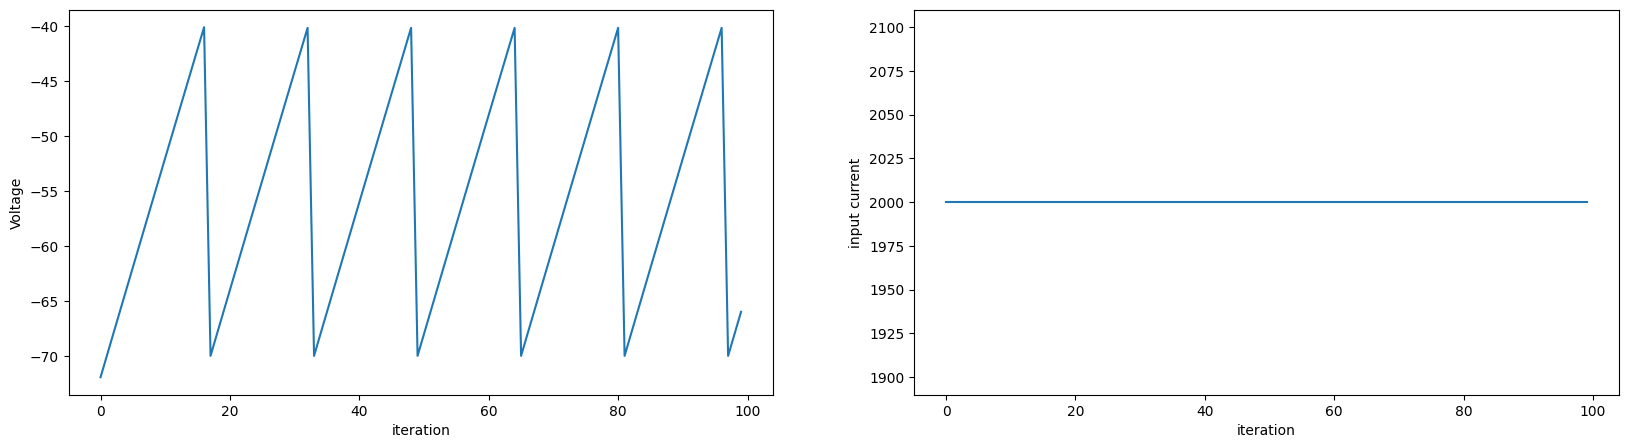
\includegraphics[width=0.9\textwidth]{Figs/lif_c.png}
\caption{تغییرات پتانسیل مدل نورونی \lr{LIF}
با جریان ثابت }
\end{figure}
\end{center}


\begin{figure}[H]
\centering
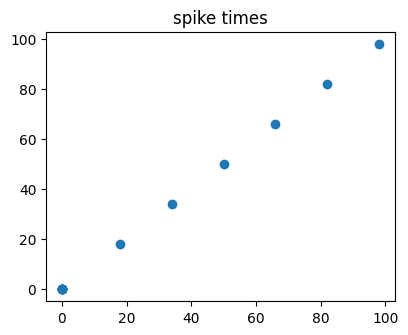
\includegraphics[width=0.4\textwidth]{Figs/lif_c_s.png}
\caption{نمودار زمان ضربه بر اساس مرحله شبیه سازی}
\label{fig:lif_c_s}
\end{figure}
\end{center}

\subsubsection*{جریان تک پله‌ای}

در این حالت همانطور که مشاهده ‌می‌کنید در ابتدا که جریان ورودی نداریم نورون با سرعت کمی شروع می‌کند تا به حالت استراحت خودش برسد اما به محض اینکه ورودی به آن می‌دهیم از انجایی که جریان ثابت است، دقیقا نورون رفتاری مشابه حالت قبل خواهد داشت و با نرح ثابتی ضربه خواهد زد.
\begin{figure}[H]
\centering
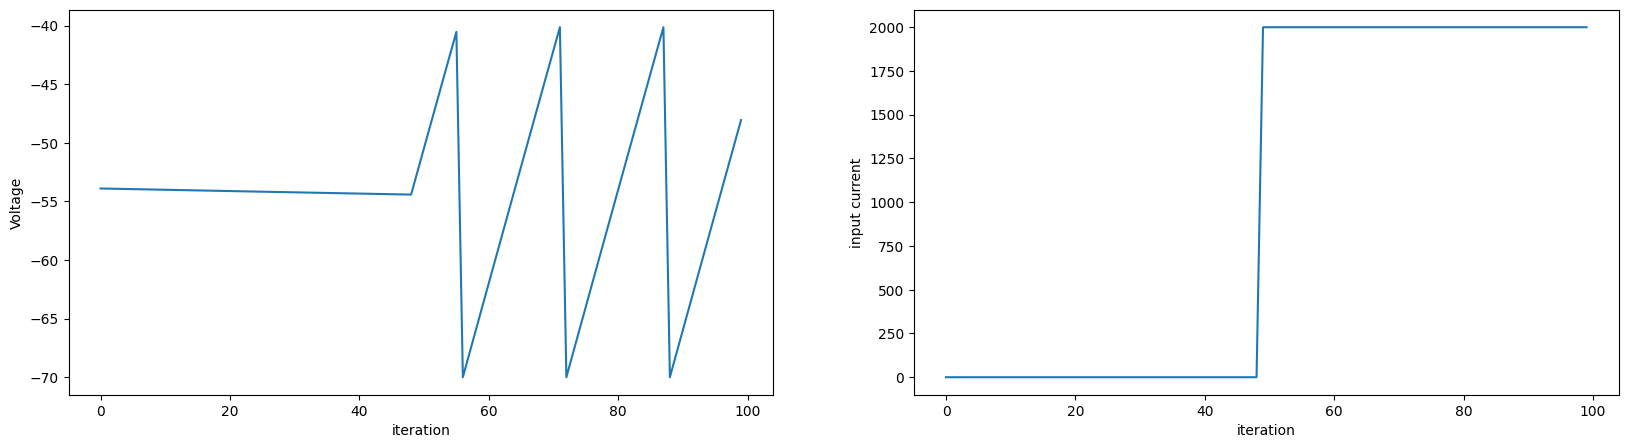
\includegraphics[width=0.9\textwidth]{Figs/lif_o_s.png}
\caption{تغییرات پتانسیل مدل نورونی \lr{LIF}
با جریان تک پله ای }
\end{figure}
\end{center}

\subsubsection*{جریان پله‌ای}
در این حالت همانطوری که مشاهده می‌کنید در گذر زمان که جریان ورودی مقدار بیشتری خواهد داشت در نتیجه با نرخ سریعتری نورون ضربه خواهد زد و هر چه که به جلوتر می‌رویم این نرخ بیشتر و بیشتر می‌شود که می‌تواند نرخ ضربه زدن را در شکل \ref{fig:lif_s_s} مشاهده کنید.

\begin{figure}[H]
\centering
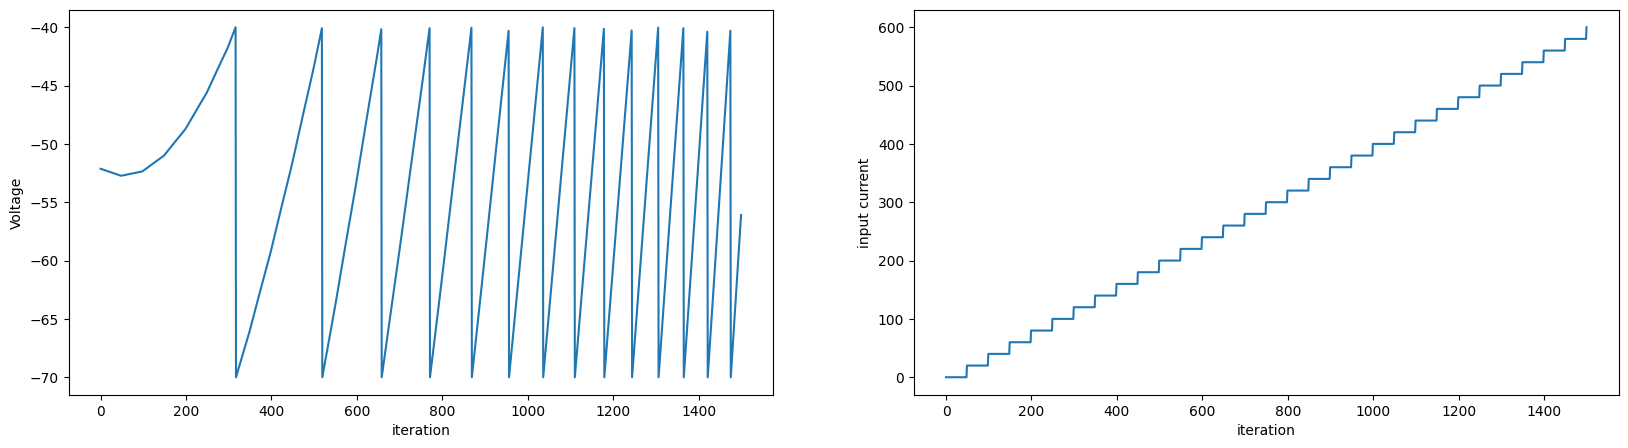
\includegraphics[width=0.9\textwidth]{Figs/lif_s.png}
\caption{تغییرات پتانسیل مدل نورونی \lr{LIF}
با جریان پله‌ای }
\end{figure}
\end{center}

\begin{figure}[H]
\centering
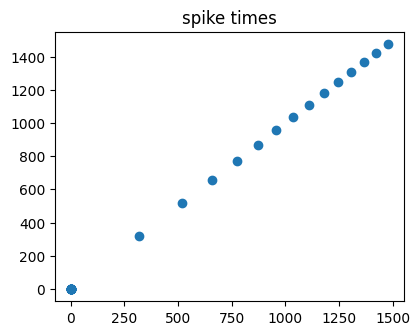
\includegraphics[width=0.4\textwidth]{Figs/lif_s_s.png}
\caption{نمودار زمان ضربه بر اساس مرحله شبیه سازی}
\label{fig:lif_s_s}
\end{figure}
\end{center}

\subsubsection*{جریان سینوسی}
در این حالت زمانی که جریان ما در حال بیشتر شدن است اختلاف پتانسل درون نورون کمتر می‌شود اما زمانی که جریان کاهشی است با نرح کمتری اختلاف پتانسیل کاهش ‌می‌یابد و با توجه به این مسئله نورون پس از چند بار افزایش جریان ضربه خواهد زد و این ضربه زدن هم چون یک مدل خطی و بدون خاصیت تطبیق پذیری داریم یک نرخ کاملا ثابت خواهد داشت.

\begin{figure}[H]
\centering
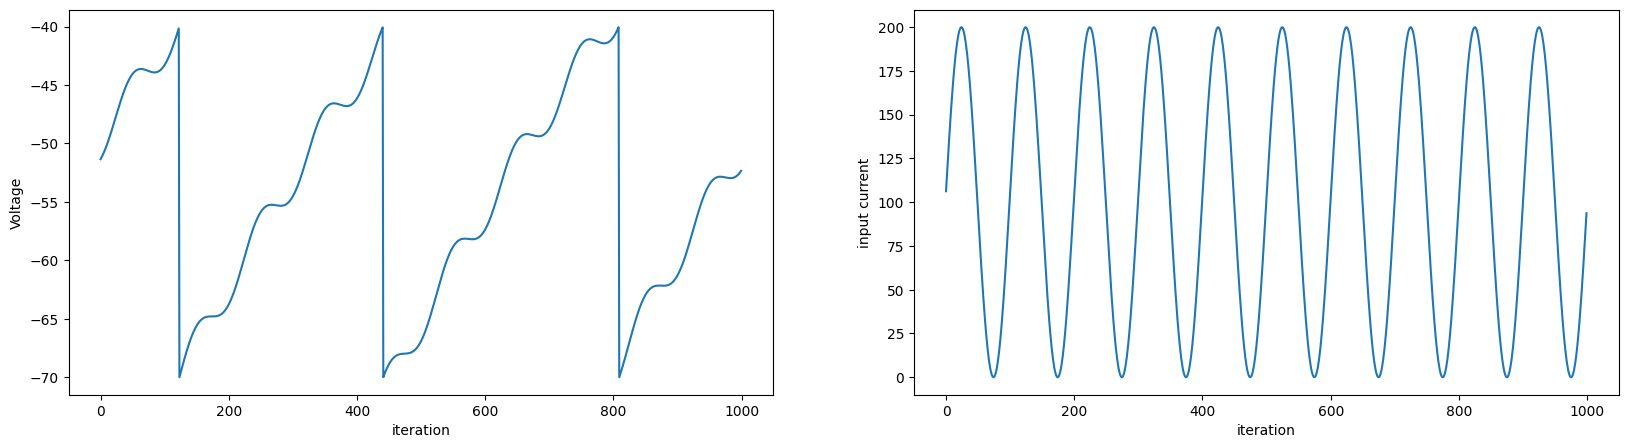
\includegraphics[width=0.9\textwidth]{Figs/lif_sin.png}
\caption{تغییرات پتانسیل مدل نورونی \lr{LIF}
با جریان سینوسی }
\end{figure}
\end{center}


%%%%%%%%%%%%%%%%%%%%%%%%%%%%%%%%%%%%%%%%%%%%%%%%%%%%%ELIF%%%%%%%%%%%%%%%%%%%%%%%%%%%%%%%%%%%%%%%
\subsection*{مدل نورونی \lr{ELIF}}	

همانطور که نتایج را برای این مدل مشاهده می‌کنید زمان های ضربه در مدل های نورونی \lr{ELIF}
کاملا مشابه مدل های نورونی \lr{LIF} است و کاملا رفتار های مشابه‌ای دارند با این تفاوت که این مدل های نورونی مکانیزم ضربه زدن های نورون های واقعی را که یک جهش در اختلاف پتانسیل آن‌ها شکل می‌گیرد در موقع ضربه را شبیه سازی می‌کند که می‌توانید آن را برای همه جریان های متفاوت مشاهده کنید، البته نکته ای که وجود دارد این است که از آنجایی که اختلاف پتانسیل نورون بعد از عبور از مقدار $\theta_{rh}$ رشد سریعی دارد و از آنجایی که در شبیه سازی رزلوشن بالایی نداریم برخی از پتانسل‌های فعالیت \LTRfootnote{action potential} به صورت کامل به نمایش گذاشته نشده‌اند.

\subsubsection*{جریان ثابت}

\begin{figure}[H]
\centering
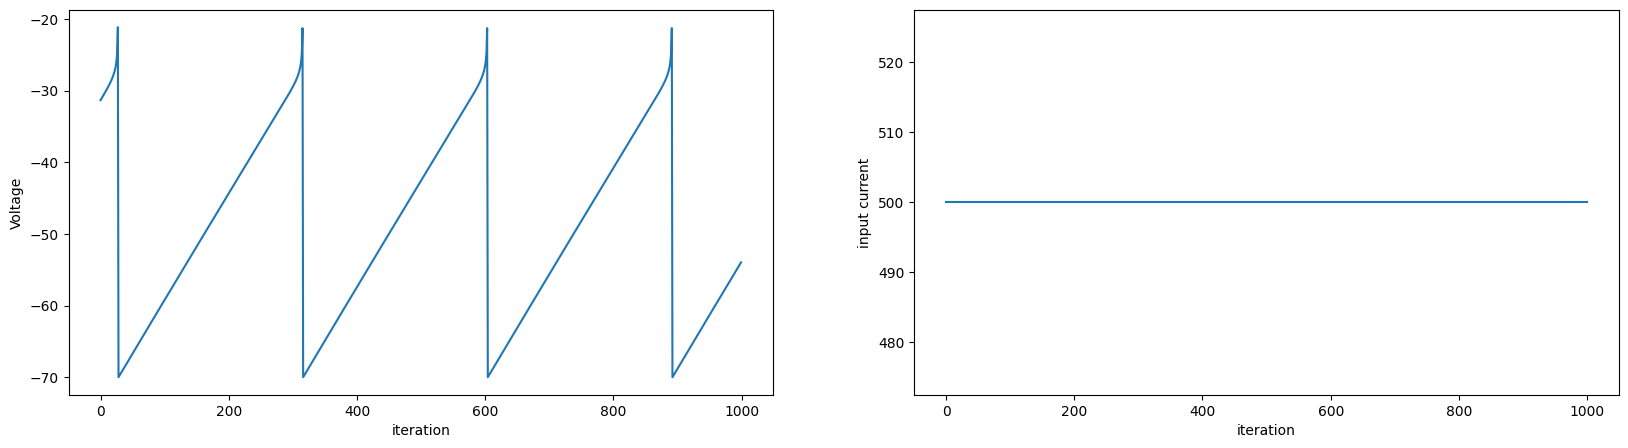
\includegraphics[width=0.9\textwidth]{Figs/elif_c.png}
\caption{تغییرات پتانسیل مدل نورونی \lr{ELIF}
با جریان ثابت }
\end{figure}
\end{center}


\subsubsection*{جریان تک پله‌ای}

\begin{figure}[H]
\centering
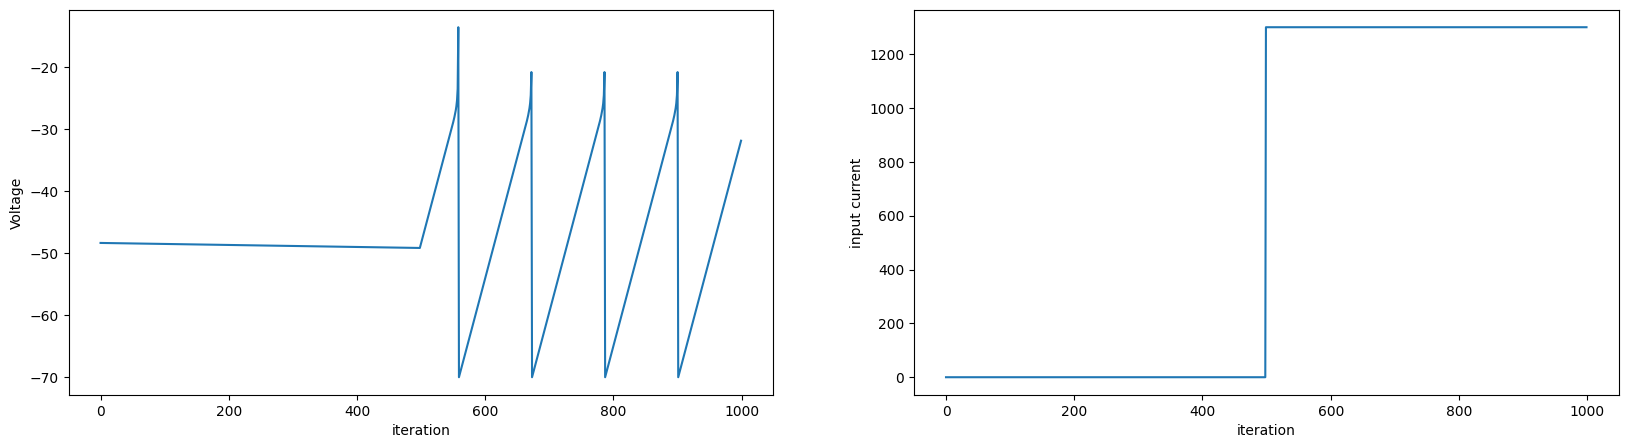
\includegraphics[width=0.9\textwidth]{Figs/elif_o_s.png}
\caption{تغییرات پتانسیل مدل نورونی \lr{ELIF}
با جریان تک پله ای }
\end{figure}
\end{center}

\subsubsection*{جریان پله‌ای}
\begin{figure}[H]
\centering
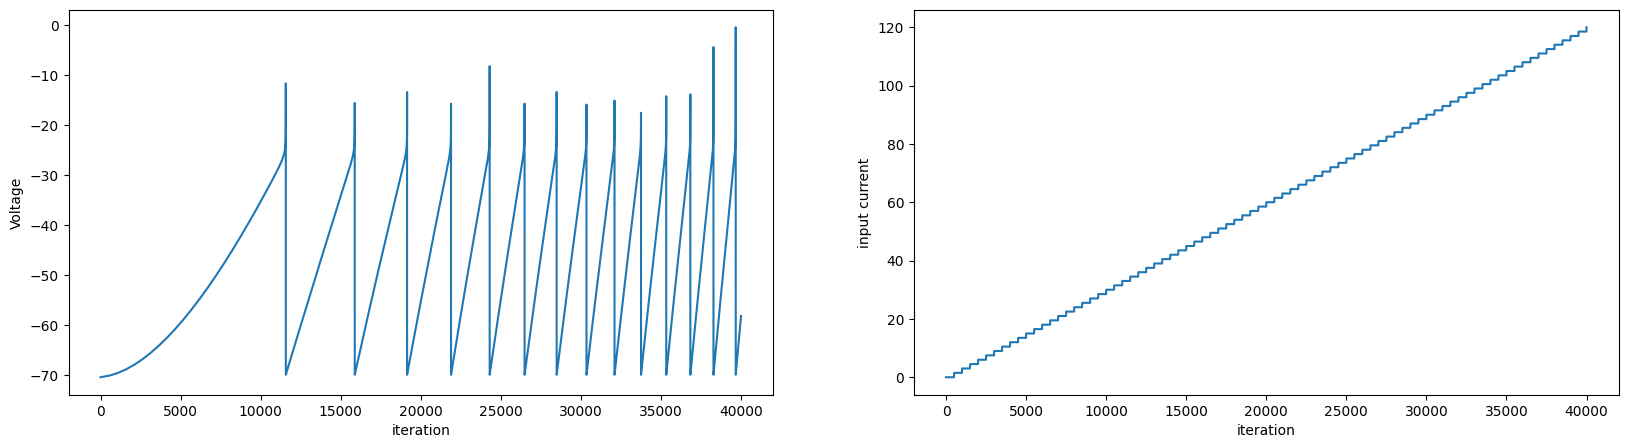
\includegraphics[width=0.9\textwidth]{Figs/elif_s.png}
\caption{تغییرات پتانسیل مدل نورونی \lr{ELIF}
با جریان پله‌ای }
\end{figure}
\end{center}

\subsubsection*{جریان سینوسی}
\begin{figure}[H]
\centering
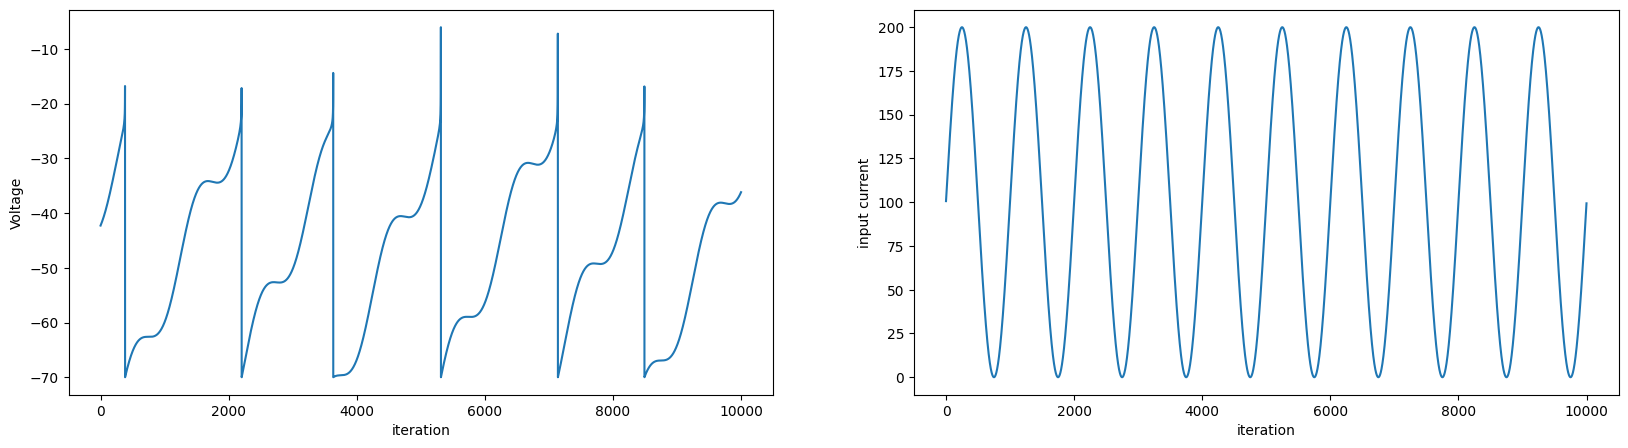
\includegraphics[width=0.9\textwidth]{Figs/elif_sin.png}
\caption{تغییرات پتانسیل مدل نورونی \lr{ELIF}
با جریان سینوسی }
\end{figure}
\end{center}
	
%%%%%%%%%%%%%%%%%%%%%%%%%%%%%%%%%%%%%%%%%%%%%%%%%%%%%AELIF%%%%%%%%%%%%%%%%%%%%%%%%%%%%%%%%%%%%%%%
\subsection*{مدل نورونی \lr{AELIF}}	
 مهمترین خصیصه و هدفی که ما در این مدل به دنبال آن بودیم شبیه سازی خاصیت تطبیق پذیری نورن ها است، نورن های واقعی بعد از اینکه ورودی ثابتی برای مدت زمان طولانی به آن ها وارد می‌شوند به آن عادت می کنند و این باعث می‌شود که میزان حساسیت آن‌ها به مرور زمان کمتر شده و البته اگر این جریان ثابت را قطع کنیم این عادت به مرور از بین خواهد رفت، پس چیزی که در این مدل باید انتظار داشته باشیم این است که رفتار تطبیق پذیری را در آن‌ها مشاهده کنیم.
\subsubsection*{جریان ثابت}
در این حالت که به نورن جریان ثابت می‌دهیم بعد از مدتی به صورت کم کم نورون ما به این ورودی عادت می‌کند و خاصیت تطبیق پذیری نورون ما باعث می‌شود که نرخ ضربه در نورون ما کاهش یابد که این را به وضوح می توانید در شکل \ref{fig:aelif_c_s} مشاهده کنید.

\begin{figure}[H]
\centering
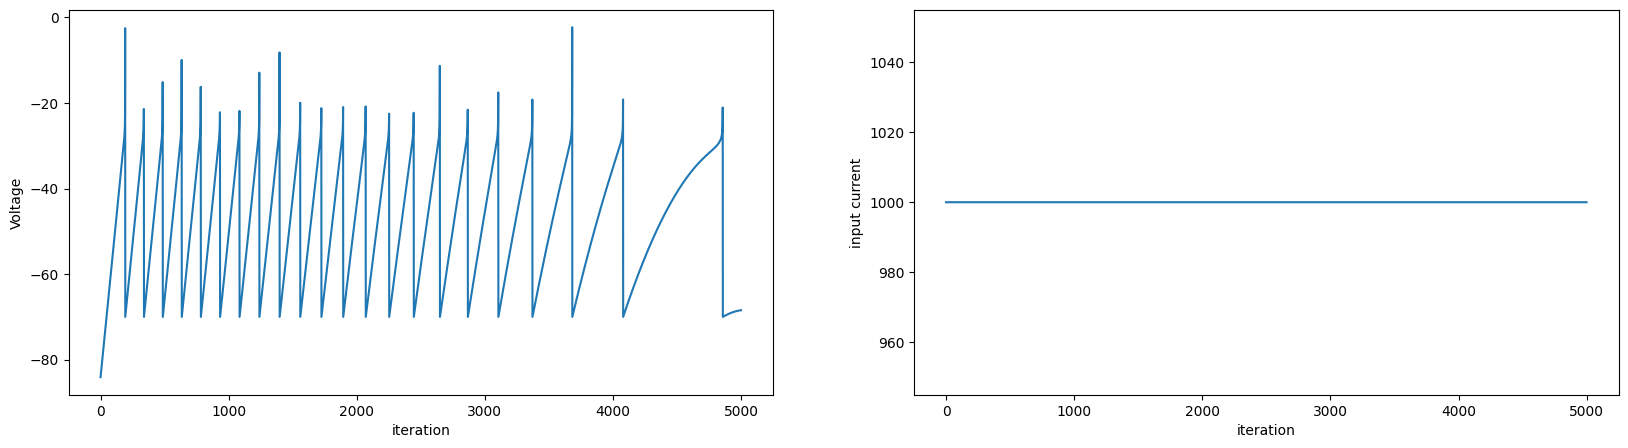
\includegraphics[width=0.9\textwidth]{Figs/aelif_c.png}
\caption{تغییرات پتانسیل مدل نورونی \lr{AELIF}
با جریان ثابت }
\end{figure}
\end{center}


\begin{figure}[H]
\centering
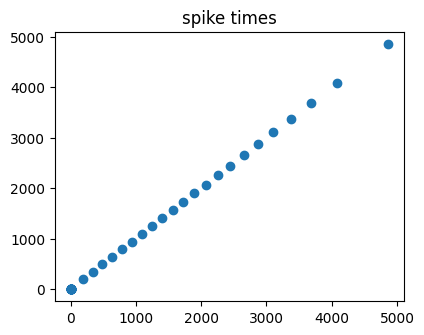
\includegraphics[width=0.4\textwidth]{Figs/aelif_c_s.png}
\caption{نمودار زمان ضربه بر اساس مرحله شبیه سازی}
\label{fig:aelif_c_s}
\end{figure}
\end{center}



\subsubsection*{جریان تک پله‌ای}
این حالت نیز تا زمانی که ورودی نداریم اختلاف پتانسیل نورون آهسته آهسته به سمت حالت استراحت می‌رود و بعد از اینکه یک جریان با نرخ ثابت وارد می‌شود مشابه قسمت قبل نورون شروع به ضربه زدن ‌می‌کند اما نرخ این ضربه ها با توجه به خاص تطبیق پذیری نورون به مرور زمان کاهش پیدا می‌کند شکل \ref{fig:aelif_o_s_s}.

\begin{figure}[H]
\centering
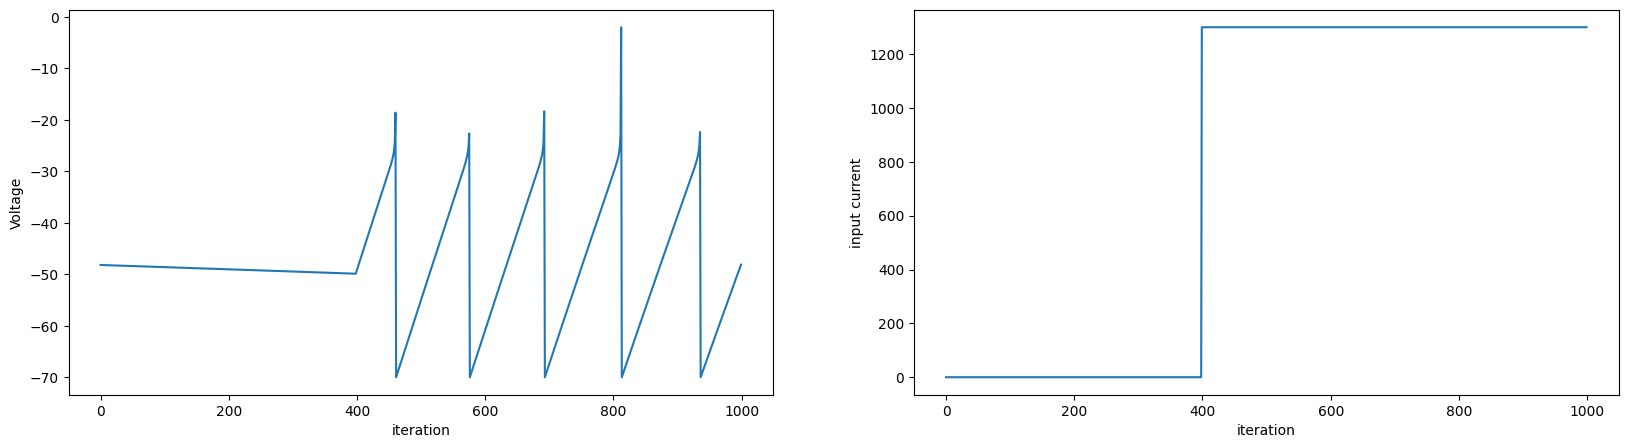
\includegraphics[width=0.9\textwidth]{Figs/aelif_o_s.png}
\caption{تغییرات پتانسیل مدل نورونی \lr{AELIF}
با جریان تک پله ای }
\end{figure}
\end{center}

\begin{figure}[H]
\centering
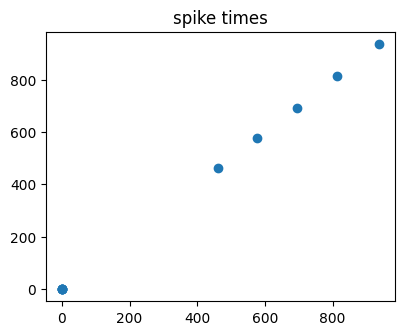
\includegraphics[width=0.4\textwidth]{Figs/aelif_o_s_s.png}
\caption{نمودار زمان ضربه بر اساس مرحله شبیه سازی}
\label{fig:aelif_o_s_s}
\end{figure}
\end{center}

\subsubsection*{جریان پله‌ای}

در این حالت جریان که مرور زمان زیاد و زیاد تر می‌شود و طبعا اختلاف پتانسیل نورون به سمت حد آستانه حرکت خواهد کرد، اما از آنجایی که خاصیت تطبیق پذیری در نورون وجود دارد باعث می‌شود نرخ ضربه زدن نورون پایین باشد.
\begin{figure}[H]
\centering
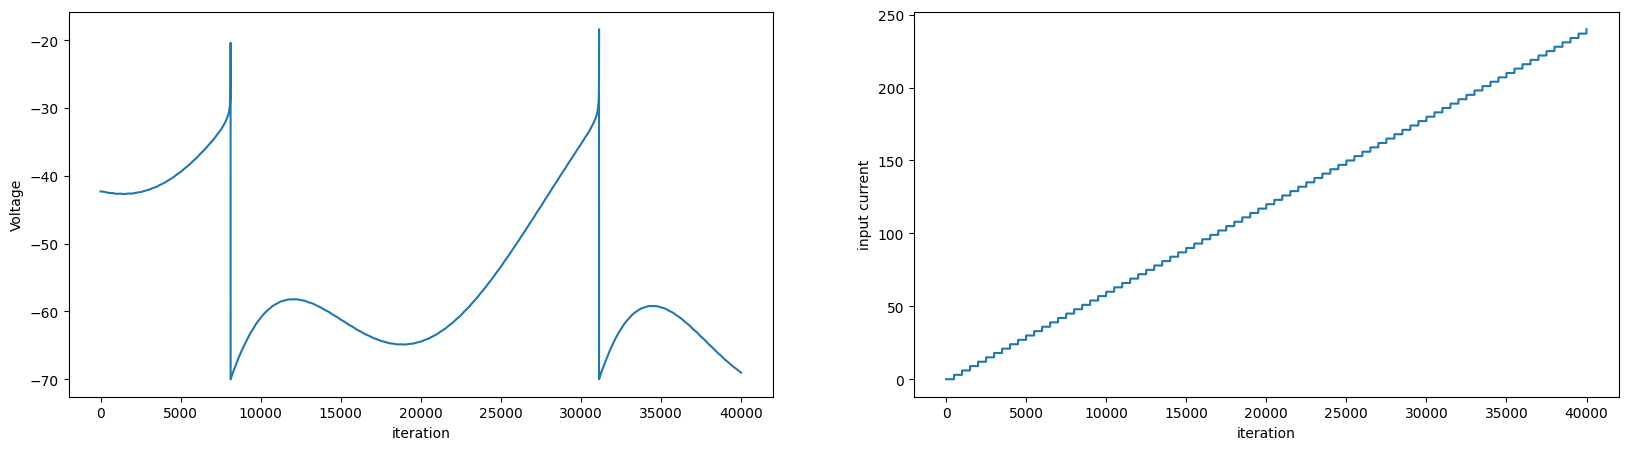
\includegraphics[width=0.9\textwidth]{Figs/aelif_s.png}
\caption{تغییرات پتانسیل مدل نورونی \lr{AELIF}
با جریان پله‌ای }
\end{figure}
\end{center}

\subsubsection*{جریان سینوسی}

در این حالت از آنجایی که جریان ما یک الگوی کاملا یکسان را طی می‌کند نورون به آن عادت می کند و از جایی به بعد اجازه نمی‌دهد نورون به راحتی وارد حالت ضربه شود و به نوعی با این ورودی مثل یک نویز برخورد خواهد کرد که نرخ ضربه آن را می‌توانید در شکل \ref{fig:aelif_sin_s} مشاهد کنید.
\begin{figure}[H]
\centering
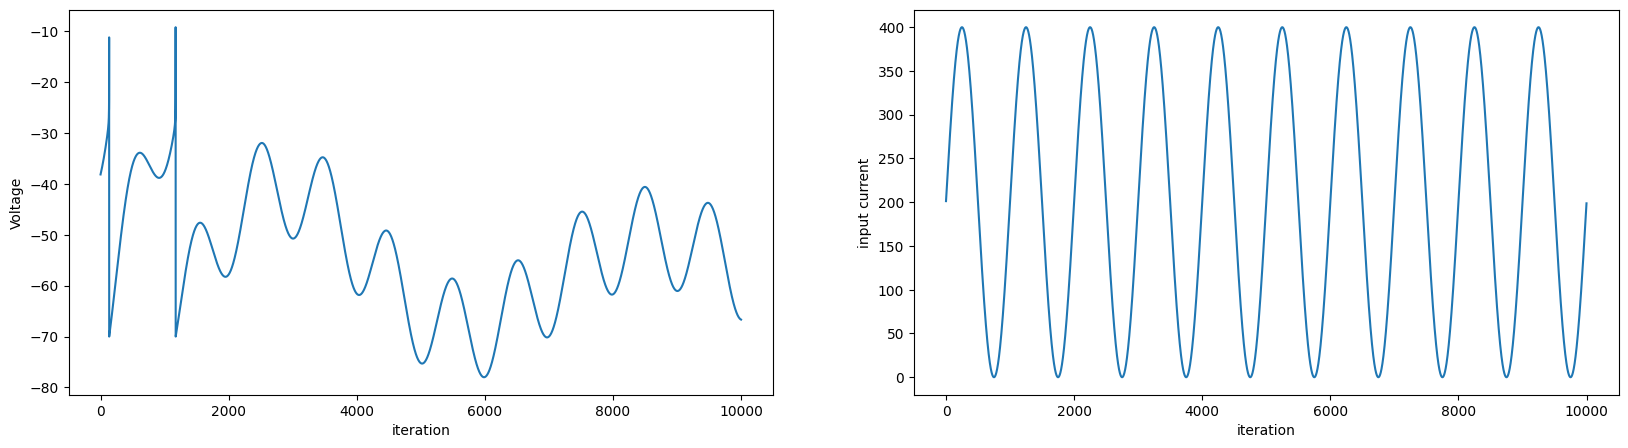
\includegraphics[width=0.9\textwidth]{Figs/aelif_sin.png}
\caption{تغییرات پتانسیل مدل نورونی \lr{AELIF}
با جریان سینوسی }
\end{figure}
\end{center}

\begin{figure}[H]
\centering
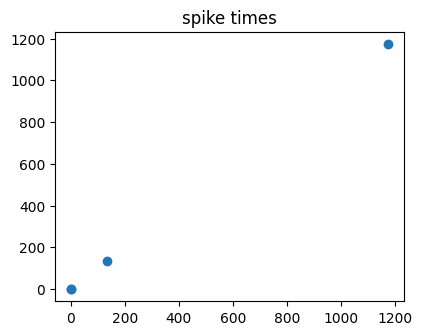
\includegraphics[width=0.4\textwidth]{Figs/aelif_sin_s.png}
\caption{نمودار زمان ضربه بر اساس مرحله شبیه سازی}
\label{fig:aelif_sin_s}
\end{figure}
\end{center}

	
\section*{ب}
در این قسمت دو جریان ورودی نویزی را پیاده کردیم که دارای توزیع های نرمال و یا یکنواخت خواهند بود، سپس  نمودار تغییرات اختلاف پتانسیل نورون‌ها را با این جریان‌ها رسم کردیم. نکته ای که وجود دارد در این حالت به یکی از جریان‌های موجود یک مقدار خاص نویز وارد نکرده‌ایم، بلکه کاملا یک جریان نویزی و رندوم را به نورون داده‌ایم و رفتار نورون را مورد بررسی قرار داده‌ایم.	

%%%%%%%%%%%%%%%%%%%%%%%%%%%%%%%%%%%%%%%%%%%%%%%%%%%%%LIF%%%%%%%%%%%%%%%%%%%%%%%%%%%%%%%%%%%%%%%
\subsection*{مدل نورونی \lr{LIF}}	

به طور کلی ازآنجایی که نرخ کاهش  اندازه اختلاف پتانسیل در این مدل نورونی کم است، ما مشاهده می کنیم که زمان هایی که جریان ها مقدار کمی دارند اندکی اندازه اختلاف پتانسیل شروع به کاهش می‌کند و اما به صورت کلی اندازه اختلاف پتانسل در حال افزایش است و در نتیجه نورون ضربه می‌زند و به طور کلی می‌توان گفت که این نورون ها با یک نرخ ثابتی ضربه می‌زنند.

\subsubsection*{جریان نویزی با توزیع نرمال}
\begin{figure}[H]
\centering
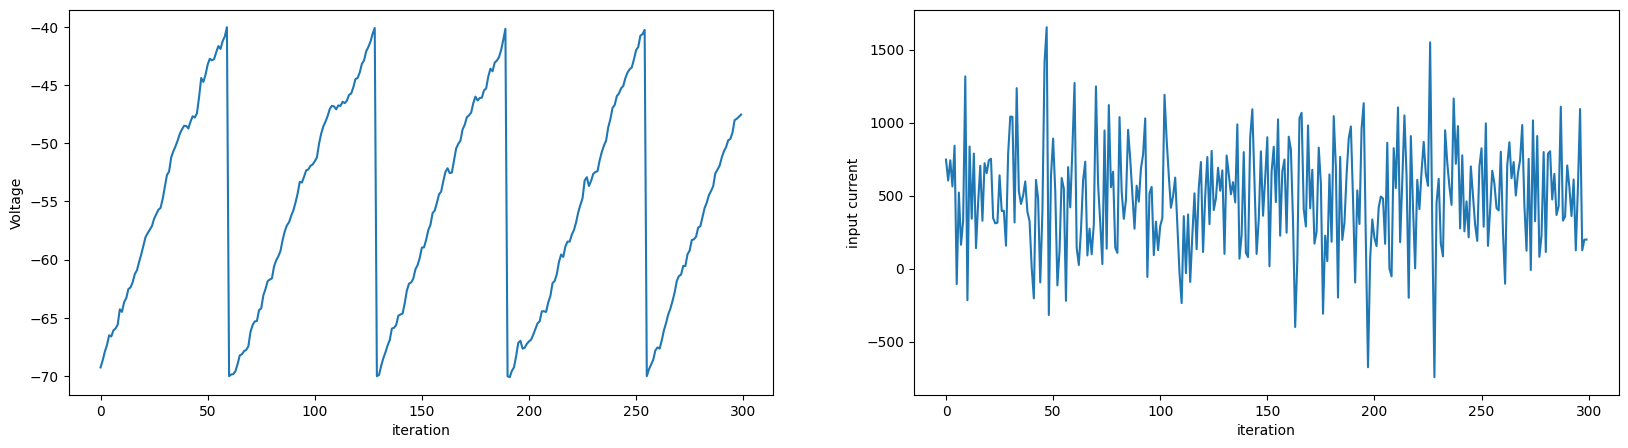
\includegraphics[width=0.9\textwidth]{Figs/lif_n_g.png}
\caption{تغییرات پتانسیل مدل نورونی \lr{LIF}
با جریان نویزی با توزیع نرمال }
\end{figure}
\end{center}

\subsubsection*{جریان نویزی با توزیع یکنواخت}
\begin{figure}[H]
\centering
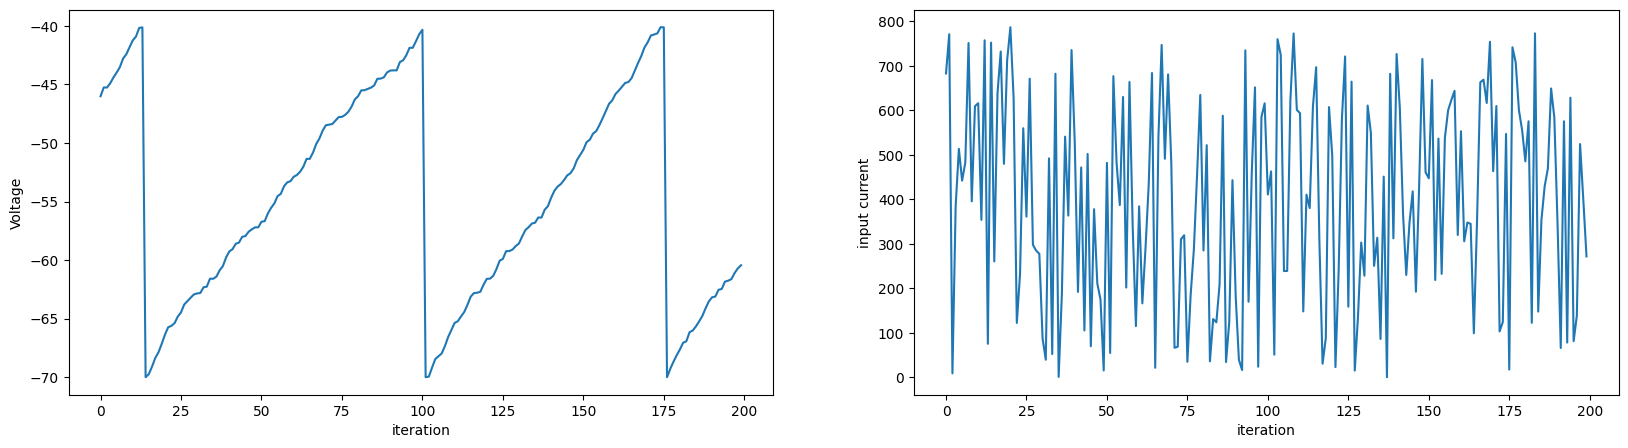
\includegraphics[width=0.9\textwidth]{Figs/lif_n_u.png}
\caption{تغییرات پتانسیل مدل نورونی \lr{LIF}
با جریان نویزی با توزیع یکنواخت }
\end{figure}
\end{center}

%%%%%%%%%%%%%%%%%%%%%%%%%%%%%%%%%%%%%%%%%%%%%%%%%%%%%ELIF%%%%%%%%%%%%%%%%%%%%%%%%%%%%%%%%%%%%%%%
\subsection*{مدل نورونی \lr{ELIF}}	
این مدل نیز دقیقا مانند مدل نورنی قبل عمل می کنند با این تفاوت که سعی می‌کنند پتانسیل فعالیت را نیز شبیه سازی کنند.
\subsubsection*{جریان نویزی با توزیع نرمال}
\begin{figure}[H]
\centering
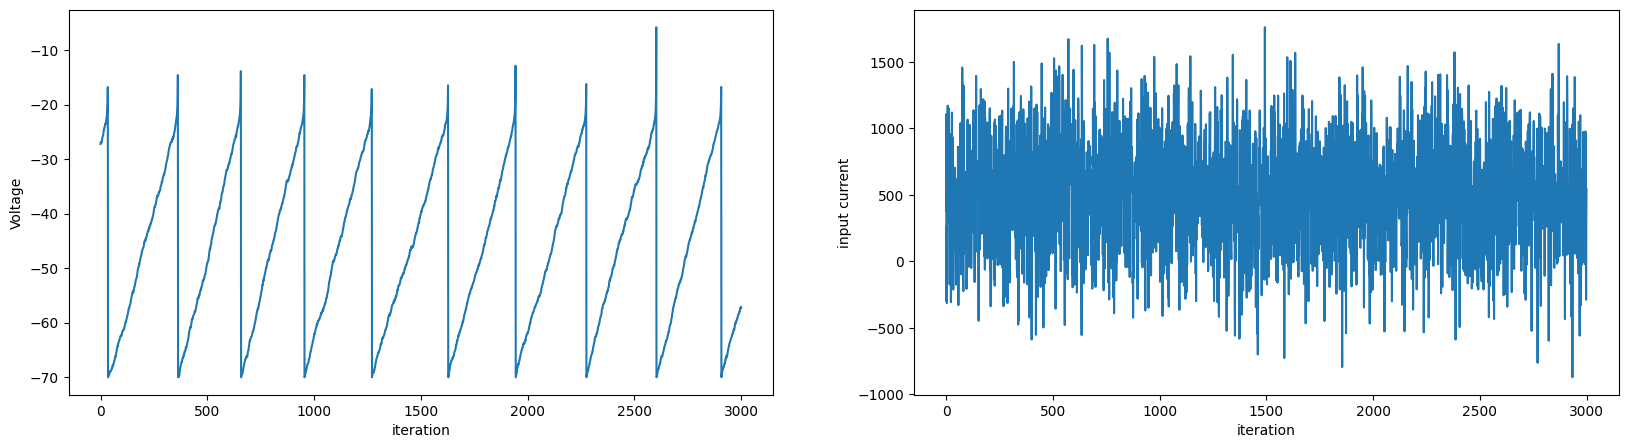
\includegraphics[width=0.9\textwidth]{Figs/elif_n_g.png}
\caption{تغییرات پتانسیل مدل نورونی \lr{ELIF}
با جریان نویزی با توزیع نرمال }
\end{figure}
\end{center}

\subsubsection*{جریان نویزی با توزیع یکنواخت}
\begin{figure}[H]
\centering
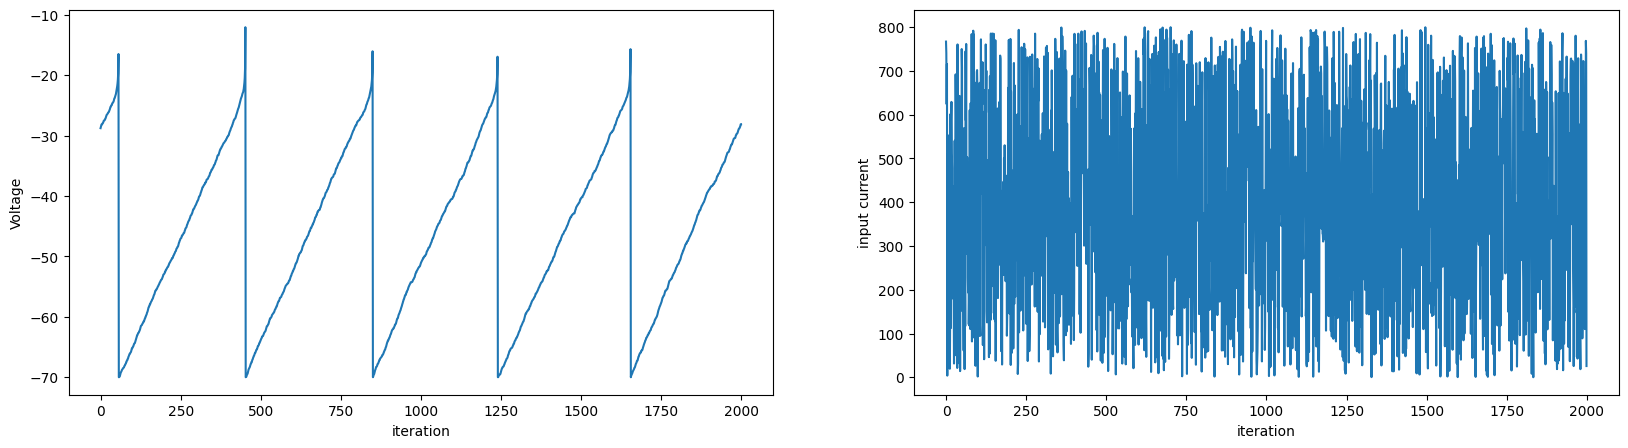
\includegraphics[width=0.9\textwidth]{Figs/elif_n_u.png}
\caption{تغییرات پتانسیل مدل نورونی \lr{ELIF}
با جریان نویزی با توزیع یکنواخت }
\end{figure}
\end{center}

%%%%%%%%%%%%%%%%%%%%%%%%%%%%%%%%%%%%%%%%%%%%%%%%%%%%%AELIF%%%%%%%%%%%%%%%%%%%%%%%%%%%%%%%%%%%%%%%
\subsection*{مدل نورونی \lr{AELIF}}	

در این مدل از آنجایی که خاصیت تطبیق پذیری را داریم مطابق انتظار بعد از مدت زمانی نورون ما به نویز وارده عادت می‌کند و با نرخ کمتری ضریه می‌زند که می‌تواند این موضوع را در شکل \ref{figs:aelif_n_g_u_s} مشاهده کنید.

\subsubsection*{جریان نویزی با توزیع نرمال}
\begin{figure}[H]
\centering
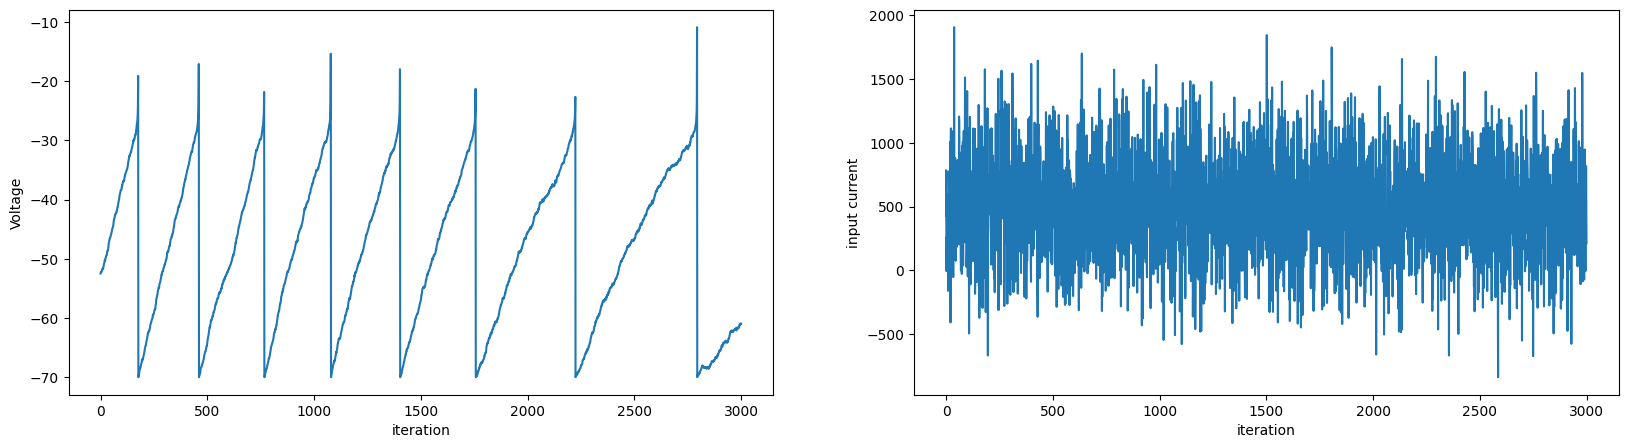
\includegraphics[width=0.9\textwidth]{Figs/aelif_n_g.png}
\caption{تغییرات پتانسیل مدل نورونی \lr{AELIF}
با جریان نویزی با توزیع نرمال }
\end{figure}
\end{center}

\subsubsection*{جریان نویزی با توزیع یکنواخت}
\begin{figure}[H]
\centering
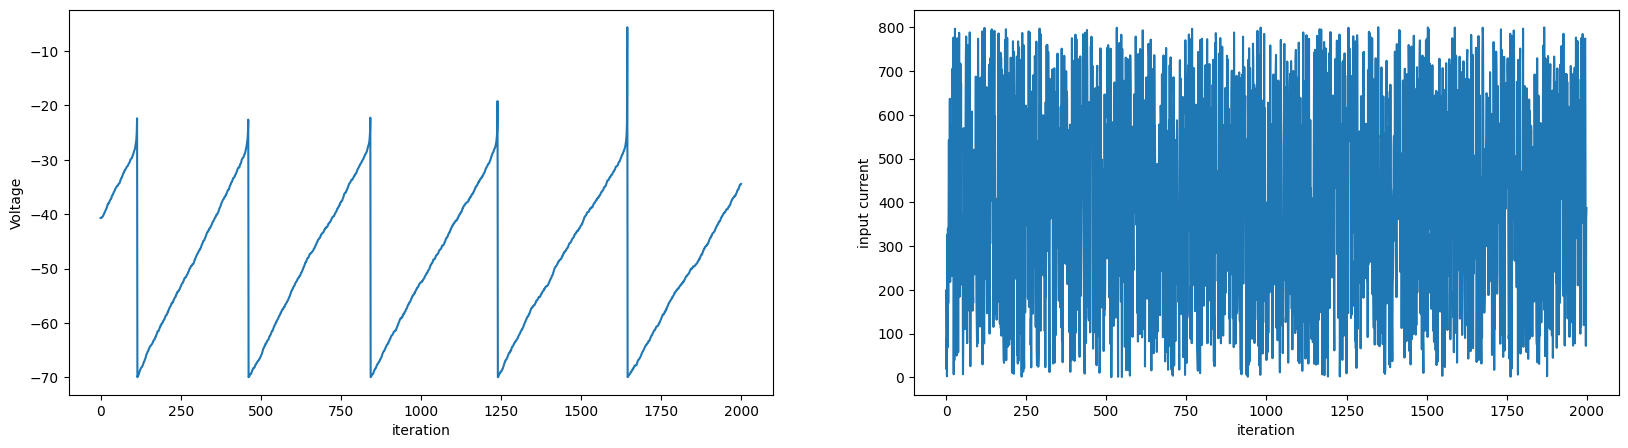
\includegraphics[width=0.9\textwidth]{Figs/aelif_n_u.png}
\caption{تغییرات پتانسیل مدل نورونی \lr{AELIF}
با جریان نویزی با توزیع یکنواخت }
\end{figure}
\end{center}

\begin{figure}[H]
\centering
  \begin{subfigure}[b]{0.4\textwidth}
    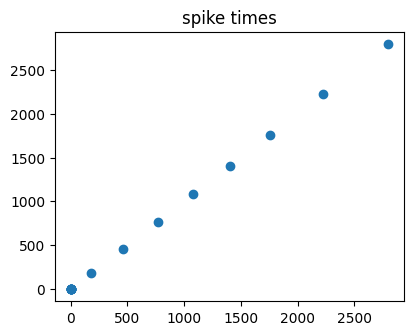
\includegraphics[width=\textwidth]{Figs/aelif_n_g_s.png}
    \caption{جریان ورودی نویزی با توزیع نرمال}
    \label{fig:f1}
  \end{subfigure}
  \hspace{3em}%
  \begin{subfigure}[b]{0.4\textwidth}
    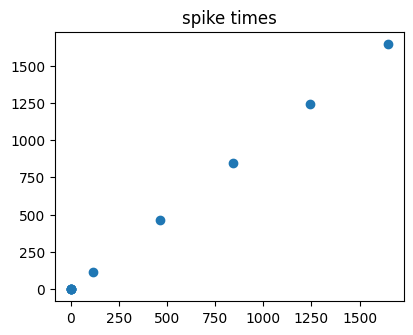
\includegraphics[width=\textwidth]{Figs/aelif_n_u_s.png}
    \caption{جریان ورودی نویزی با توزیع یکنواخت}
    \label{fig:f2}
  \end{subfigure}
  \caption{نرخ ضربه برای مدل نورنی \lr{AELIF}}
  \label{figs:aelif_n_g_u_s}
\end{figure}
\end{center}


\section*{ج} 
برای هر یک از مدل‌های نورونی با استفاده از جریان‌های ثابت متفاوت، فرکانس را اندازه می‌گیریم و در نهایت نتایج به عنوان نمودار ارائه می‌دهیم. 

\textbf{نکته مهم}: ما فرکانس را نسبت تعداد کل ضربه ها به تعداد مراحل شبیه سازی در نظر گرفته ایم.

\begin{figure}[H]
\centering
  \begin{subfigure}[b]{0.4\textwidth}
    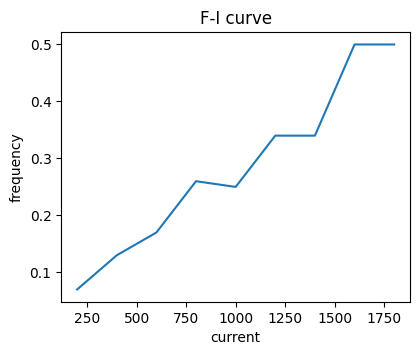
\includegraphics[width=\textwidth]{Figs/lif_f_i.png}
    \caption{جریان ثابت بدون نویز}
  \end{subfigure}
  \hspace{3em}%
  \begin{subfigure}[b]{0.4\textwidth}
    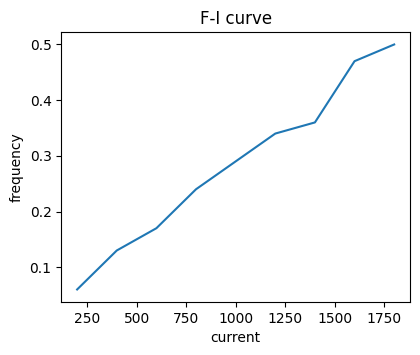
\includegraphics[width=\textwidth]{Figs/lif_f_i_n.png}
    \caption{جریان ثابت با نویز نرمال}
  \end{subfigure}
  \caption{نمودار جریان-فرکانس برای مدل نورنی \lr{LIF}}
\end{figure}
\end{center}


\begin{figure}[H]
\centering
  \begin{subfigure}[b]{0.4\textwidth}
    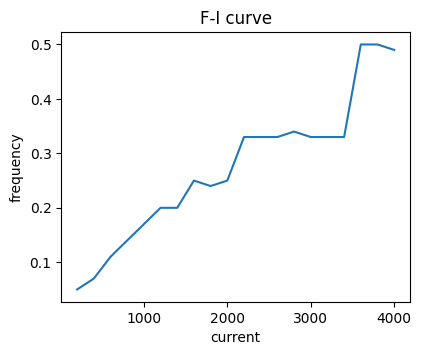
\includegraphics[width=\textwidth]{Figs/elif_f_i.png}
    \caption{جریان ثابت بدون نویز}
  \end{subfigure}
  \hspace{3em}%
  \begin{subfigure}[b]{0.4\textwidth}
    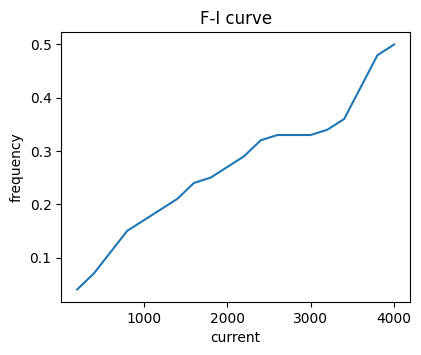
\includegraphics[width=\textwidth]{Figs/elif_f_i_n.png}
    \caption{جریان ثابت با نویز نرمال}
  \end{subfigure}
  \caption{نمودار جریان-فرکانس برای مدل نورنی \lr{ELIF}}
\end{figure}
\end{center}

\begin{figure}[H]
\centering
  \begin{subfigure}[b]{0.4\textwidth}
    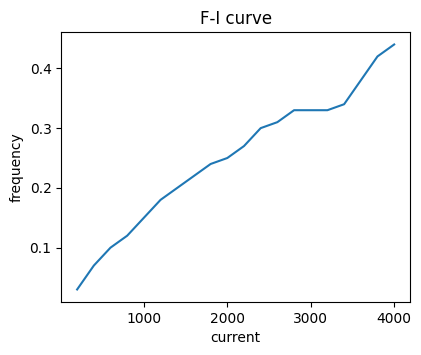
\includegraphics[width=\textwidth]{Figs/aelif_f_i.png}
    \caption{جریان ثابت بدون نویز}
  \end{subfigure}
  \hspace{3em}%
  \begin{subfigure}[b]{0.4\textwidth}
    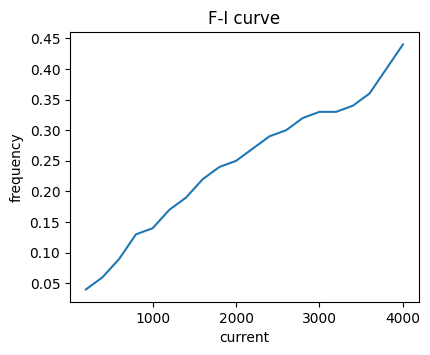
\includegraphics[width=\textwidth]{Figs/aelif_f_i_n.png}
    \caption{جریان ثابت با نویز نرمال}
  \end{subfigure}
  \caption{نمودار جریان-فرکانس برای مدل نورنی \lr{AELIF}}
\end{figure}
\end{center}

همانطور که در همه مدل‌ها مشاهده می‌کنید، زمانی که به نورون نویز وارد می‌کنیمِ، نمودار جریان-فرکانس حاصل صاف‌تر و هموارتر\LTRfootnote{Smooth} خواهد بود به طوری که هر چه میزان این نویز بیشتر باشد، نمودار صاف تر است و مانند $y = x$ می‌شود، در صورتی که وقتی جریان نویزی نیست، تابع ما بیشتر شکل پله‌ای دارد و با افزایش جریان به صورت پله‌ای فرکانس زیاد می‌شود. البته در مدل نورونی \lr{AELIF} از آنجایی که خاصیت تطبیق پذیری داریم، مدل ما به نویز حساسیت کمتری دارد، پس خیلی تغییر زیادی حس نخواهیم کرد و در حالتی که نویز وارد کردیم و بدون نویز بودیم تفاوت چندانی در رفتار نورون نمی‌توان مشاهده کرد مگر اینکه مقدار نویز را خیلی بیشتر کنیم.

\section*{د}
برای افزودن \lr{Refactory}
بعد از هر ضربه تا یک مدت زمان مشخص جریان ورودی را قطع می‌کنیم تا این فرآیند شبیه سازی شود، که نتایج آن را برای تمامی مدل‌ها و ورودی‌هایی که تا به این لحظه ارائه دادیم به نمایش خواهیم گذاشت:

%%%%%%%%%%%%%%%%%%%%%%%%%%%%%%%%%%%%%%%%%%%%%%%%%%%%%LIF%%%%%%%%%%%%%%%%%%%%%%%%%%%%%%%%%%%%%%%
\subsection*{مدل نورونی \lr{LIF}}	
\begin{figure}[H]
\centering
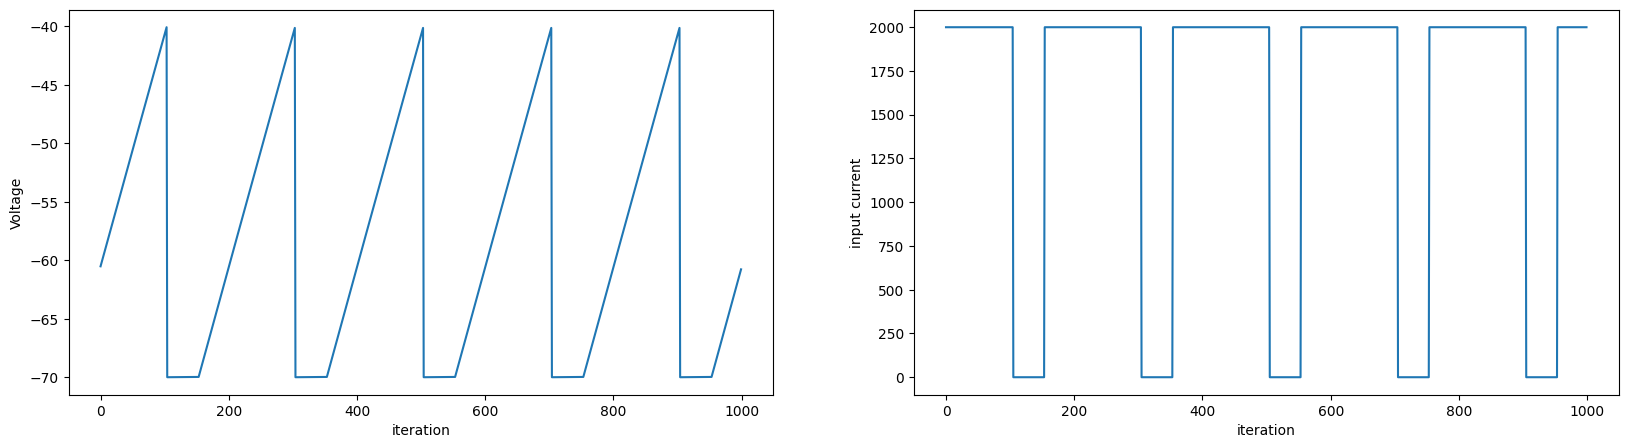
\includegraphics[width=0.9\textwidth]{Figs/lif_c_r.png}
\caption{تغییرات پتانسیل مدل نورونی \lr{LIF}
با جریان ثابت }
\end{figure}
\end{center}


\begin{figure}[H]
\centering
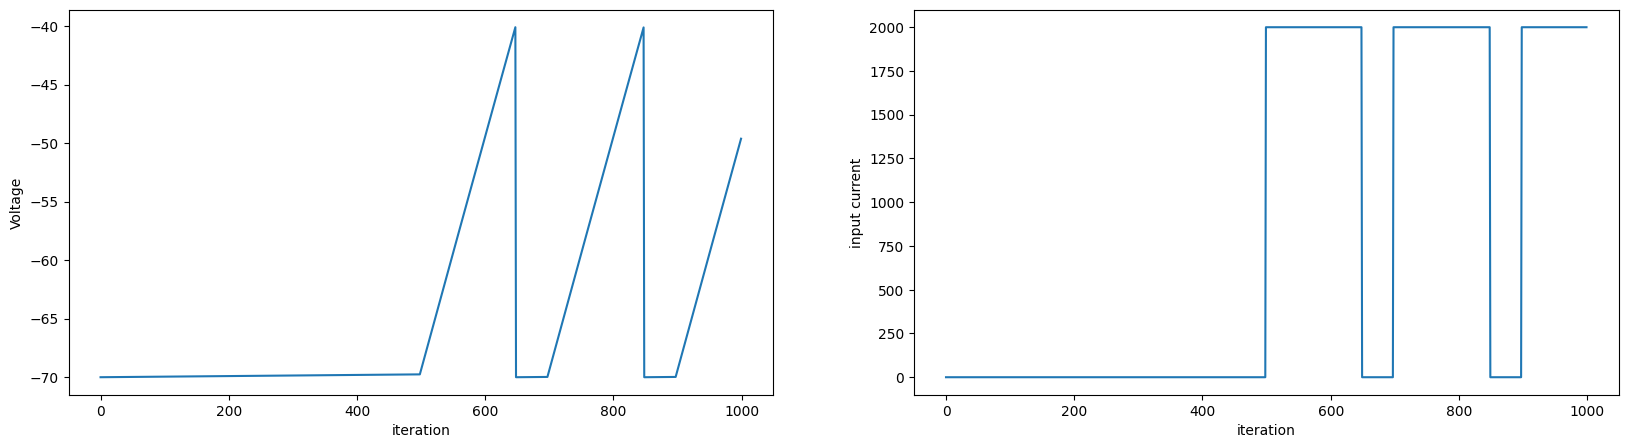
\includegraphics[width=0.9\textwidth]{Figs/lif_o_s_r.png}
\caption{تغییرات پتانسیل مدل نورونی \lr{LIF}
با جریان تک پله ای }
\end{figure}
\end{center}


\begin{figure}[H]
\centering
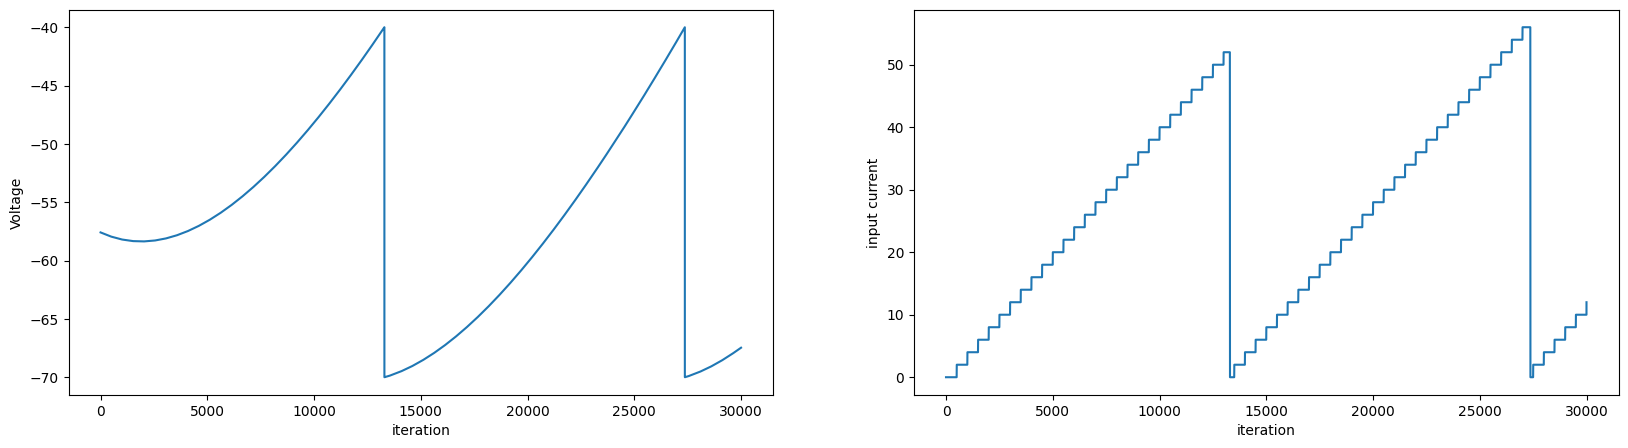
\includegraphics[width=0.9\textwidth]{Figs/lif_s_r.png}
\caption{تغییرات پتانسیل مدل نورونی \lr{LIF}
با جریان پله‌ای }
\end{figure}
\end{center}


\begin{figure}[H]
\centering
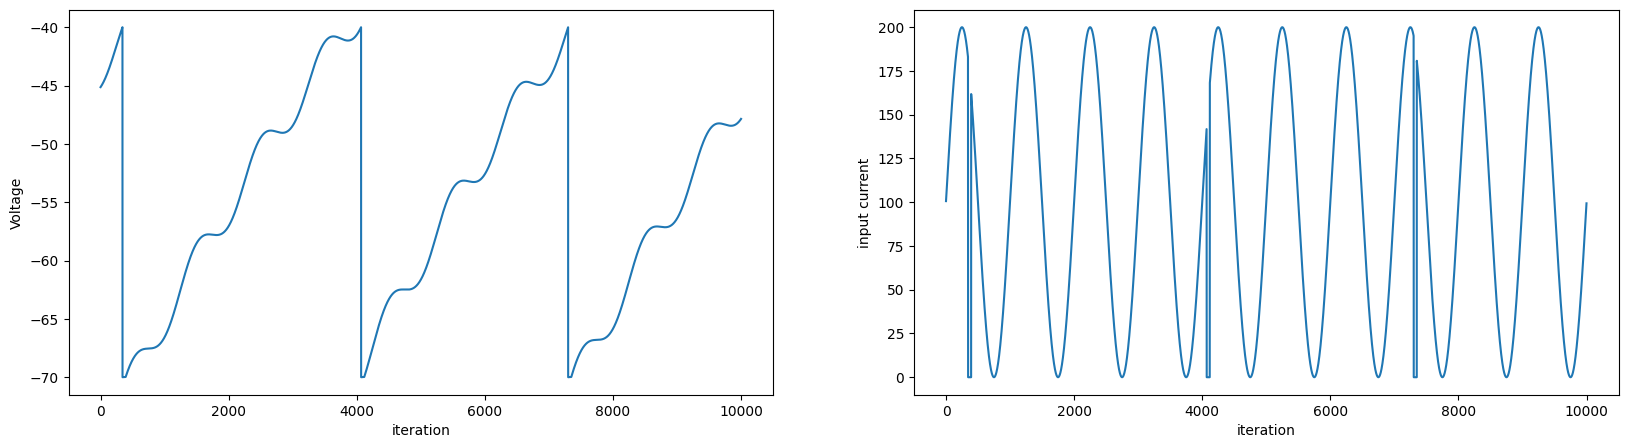
\includegraphics[width=0.9\textwidth]{Figs/lif_sin_r.png}
\caption{تغییرات پتانسیل مدل نورونی \lr{LIF}
با جریان سینوسی }
\end{figure}
\end{center}


\begin{figure}[H]
\centering
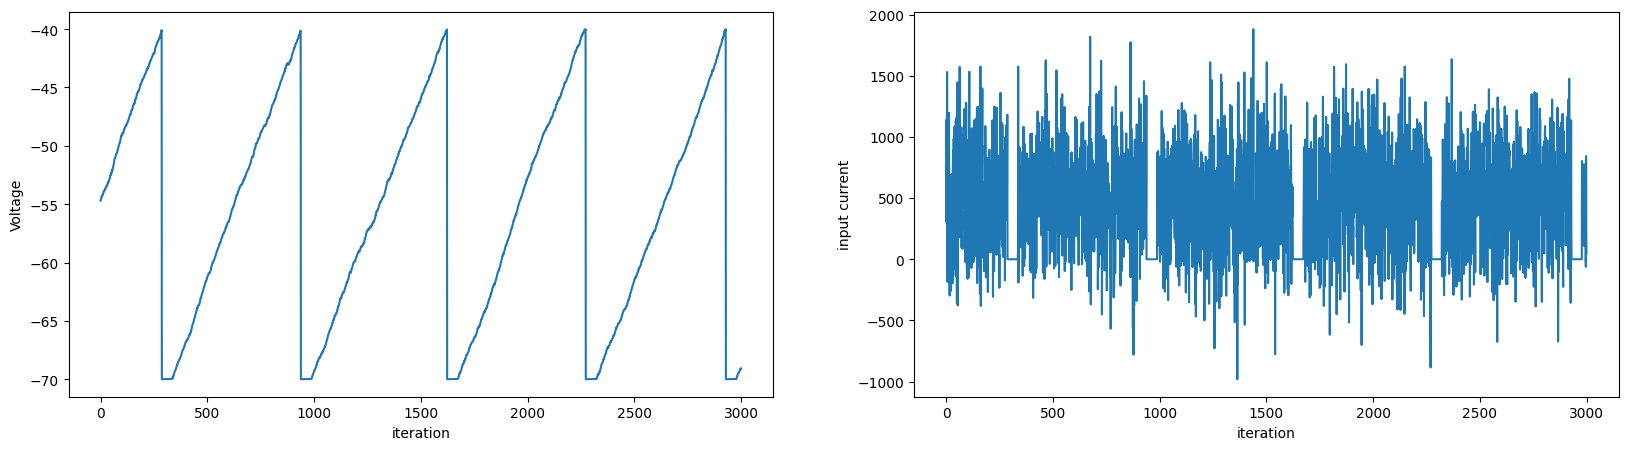
\includegraphics[width=0.9\textwidth]{Figs/lif_n_g_r.png}
\caption{تغییرات پتانسیل مدل نورونی \lr{LIF}
با جریان نویزی با توزیع نرمال }
\end{figure}
\end{center}


\begin{figure}[H]
\centering
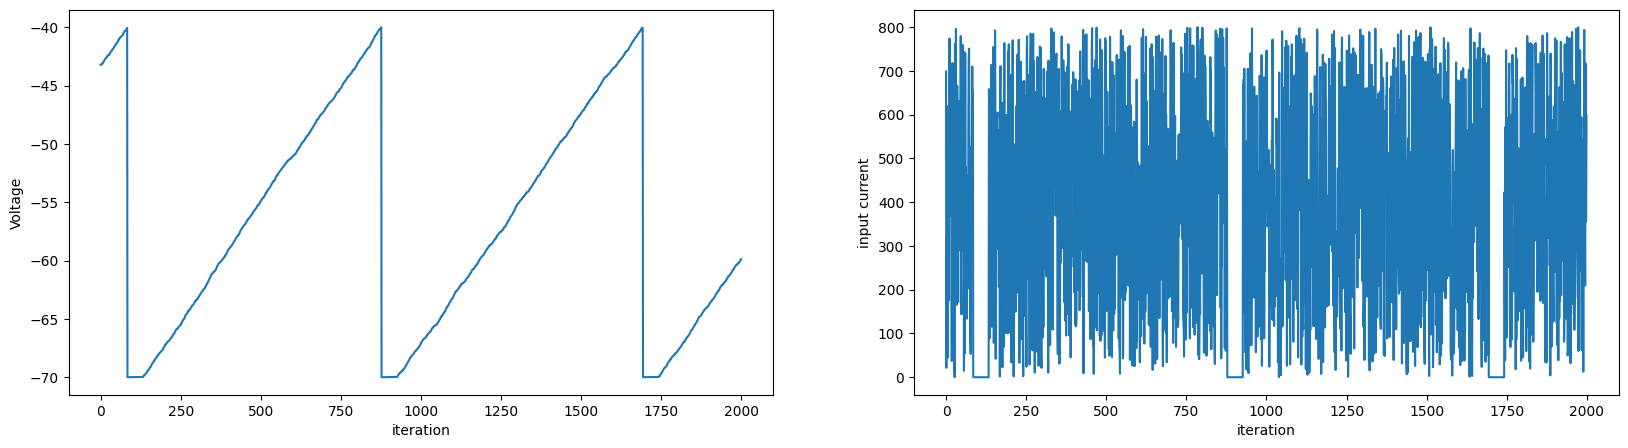
\includegraphics[width=0.9\textwidth]{Figs/lif_n_u_r.png}
\caption{تغییرات پتانسیل مدل نورونی \lr{LIF}
با جریان نویزی با توزیع یکنواخت }
\end{figure}
\end{center}

%%%%%%%%%%%%%%%%%%%%%%%%%%%%%%%%%%%%%%%%%%%%%%%%%%%%%ELIF%%%%%%%%%%%%%%%%%%%%%%%%%%%%%%%%%%%%%%%
\subsection*{مدل نورونی \lr{ELIF}}	
\begin{figure}[H]
\centering
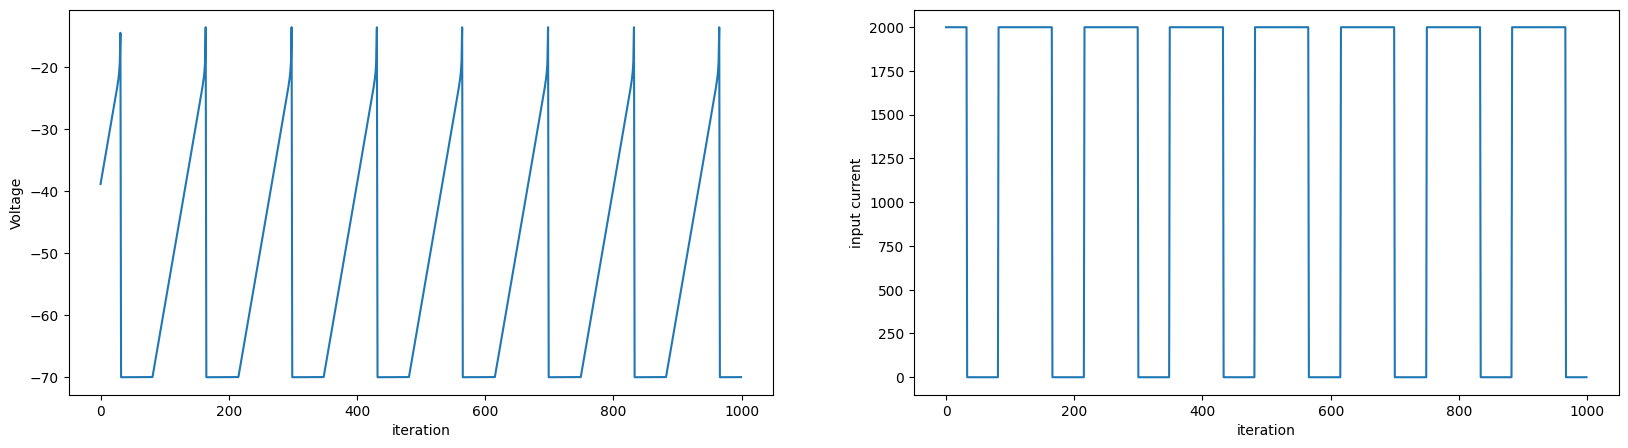
\includegraphics[width=0.9\textwidth]{Figs/elif_c_r.png}
\caption{تغییرات پتانسیل مدل نورونی \lr{ELIF}
با جریان ثابت }
\end{figure}
\end{center}


\begin{figure}[H]
\centering
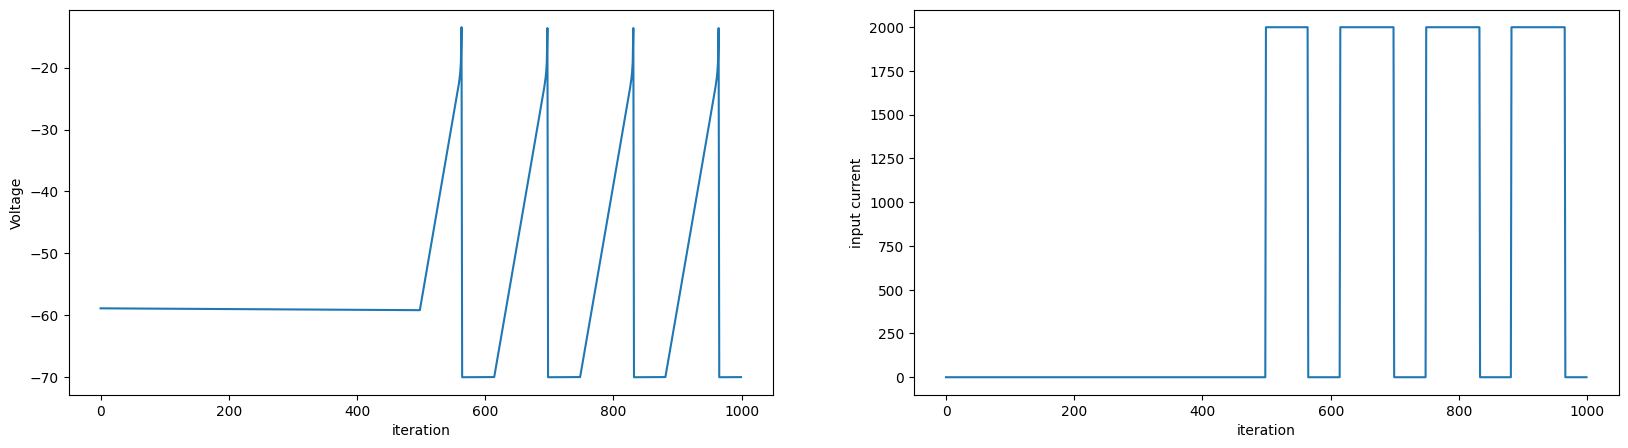
\includegraphics[width=0.9\textwidth]{Figs/elif_o_s_r.png}
\caption{تغییرات پتانسیل مدل نورونی \lr{ELIF}
با جریان تک پله ای }
\end{figure}
\end{center}


\begin{figure}[H]
\centering
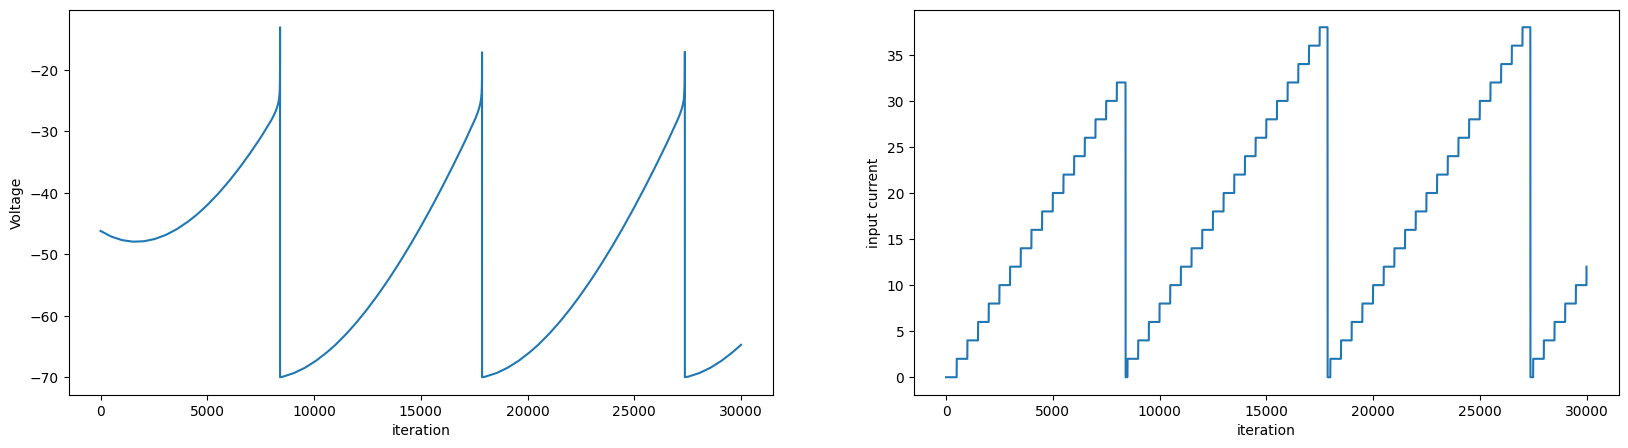
\includegraphics[width=0.9\textwidth]{Figs/elif_s_r.png}
\caption{تغییرات پتانسیل مدل نورونی \lr{ELIF}
با جریان پله‌ای }
\end{figure}
\end{center}


\begin{figure}[H]
\centering
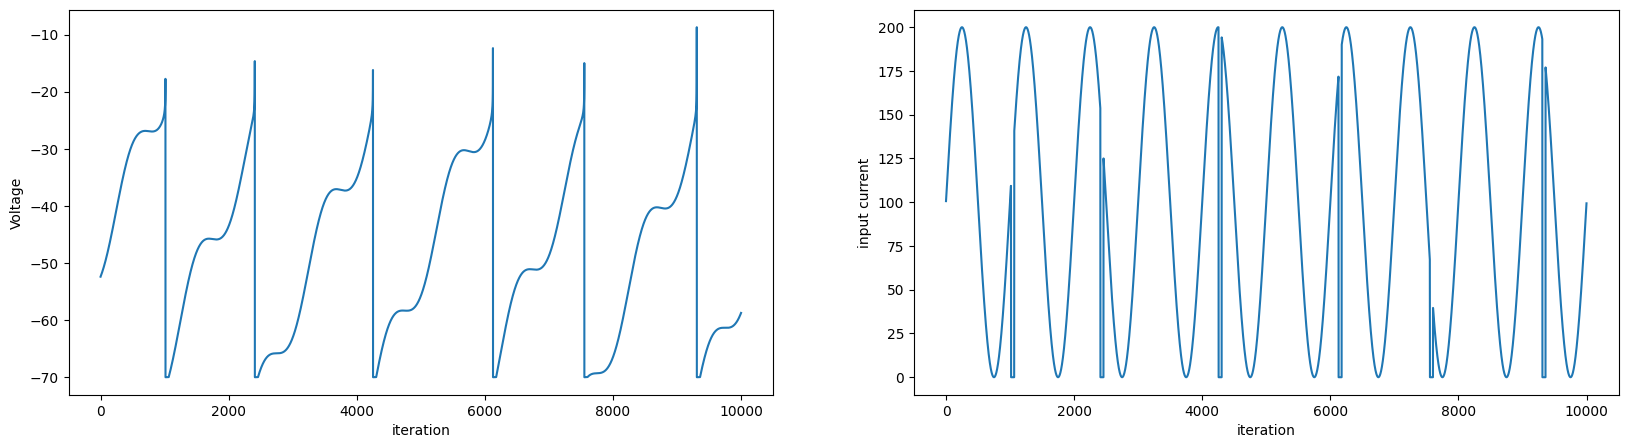
\includegraphics[width=0.9\textwidth]{Figs/elif_sin_r.png}
\caption{تغییرات پتانسیل مدل نورونی \lr{ELIF}
با جریان سینوسی }
\end{figure}
\end{center}
	
\begin{figure}[H]
\centering
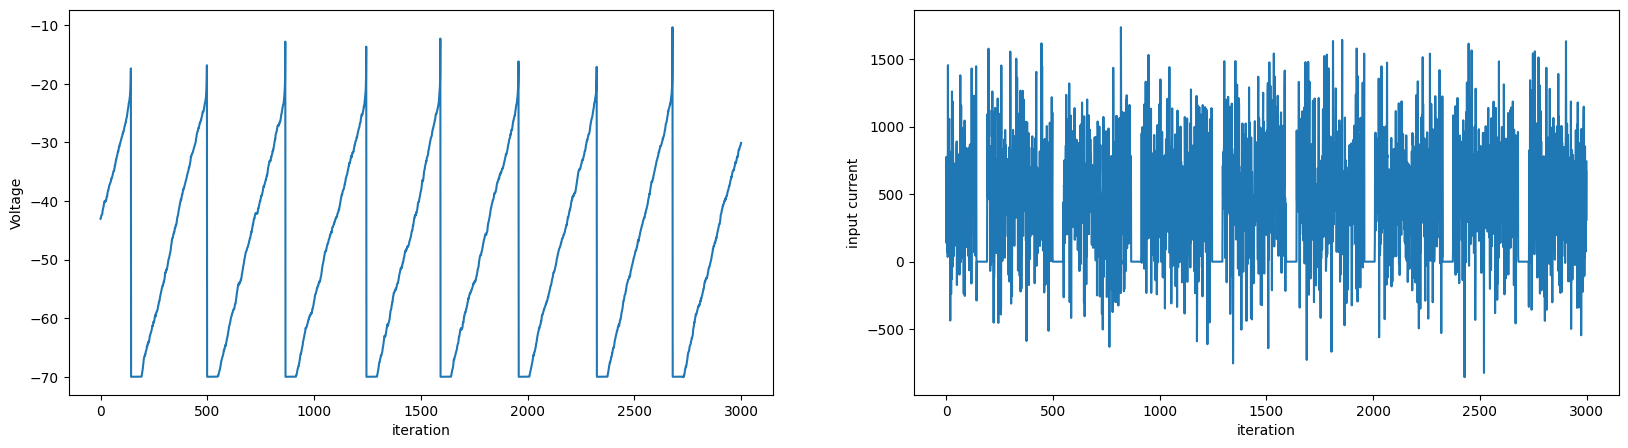
\includegraphics[width=0.9\textwidth]{Figs/elif_n_g_r.png}
\caption{تغییرات پتانسیل مدل نورونی \lr{ELIF}
با جریان نویزی با توزیع نرمال }
\end{figure}
\end{center}


\begin{figure}[H]
\centering
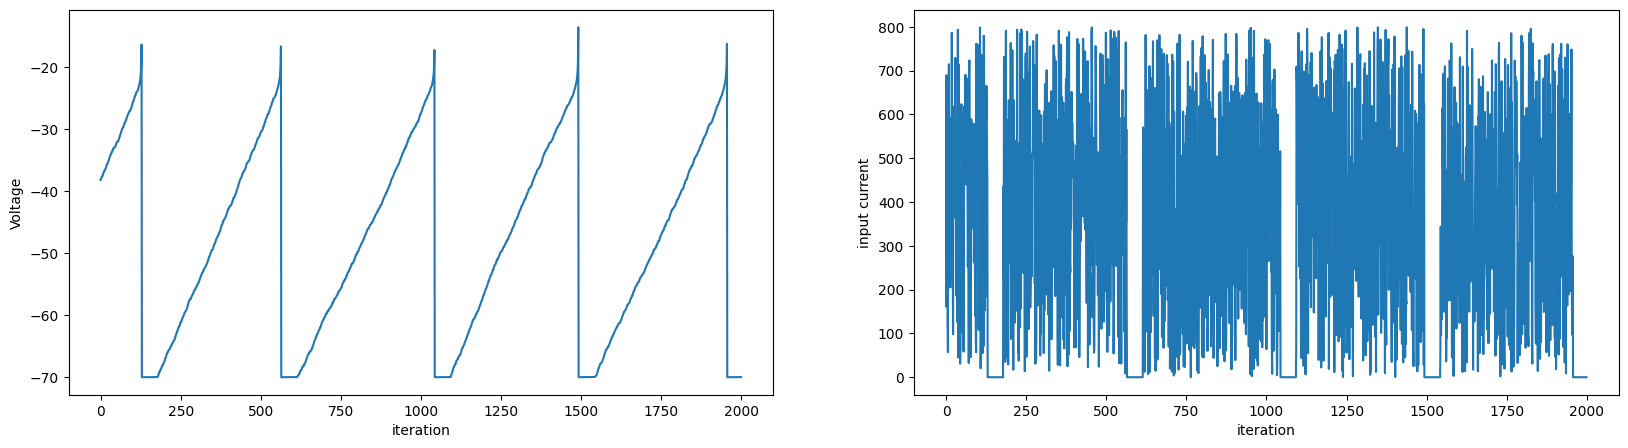
\includegraphics[width=0.9\textwidth]{Figs/elif_n_u_r.png}
\caption{تغییرات پتانسیل مدل نورونی \lr{ELIF}
با جریان نویزی با توزیع یکنواخت }
\end{figure}
\end{center}
	
%%%%%%%%%%%%%%%%%%%%%%%%%%%%%%%%%%%%%%%%%%%%%%%%%%%%%AELIF%%%%%%%%%%%%%%%%%%%%%%%%%%%%%%%%%%%%%%%
\subsection*{مدل نورونی \lr{AELIF}}	
\begin{figure}[H]
\centering
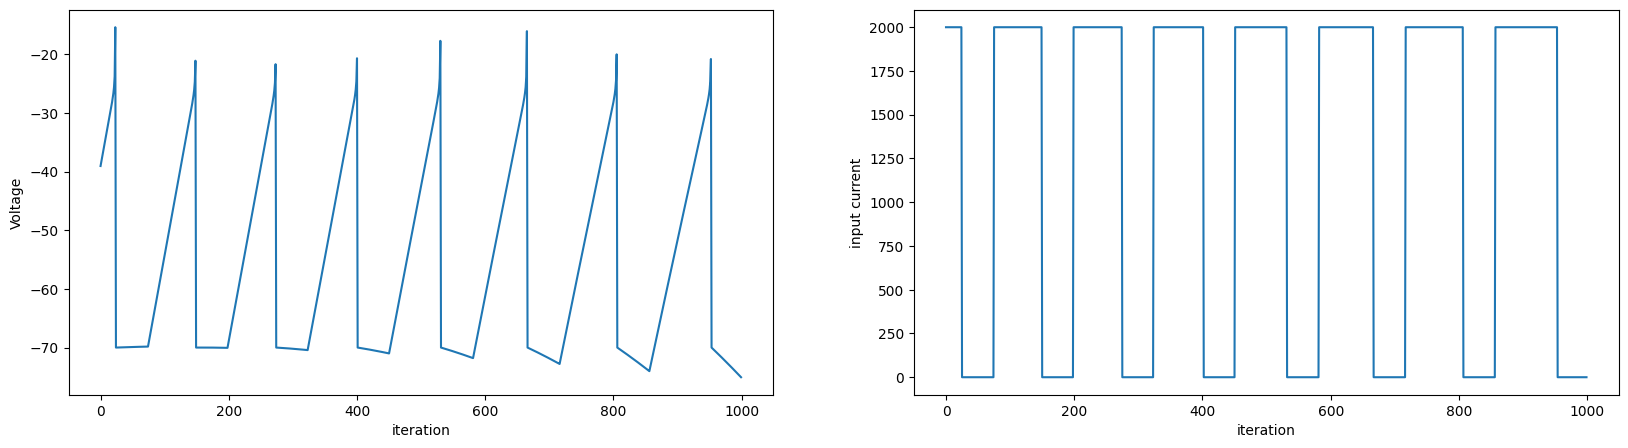
\includegraphics[width=0.9\textwidth]{Figs/aelif_c_r.png}
\caption{تغییرات پتانسیل مدل نورونی \lr{AELIF}
با جریان ثابت }
\end{figure}
\end{center}


\begin{figure}[H]
\centering
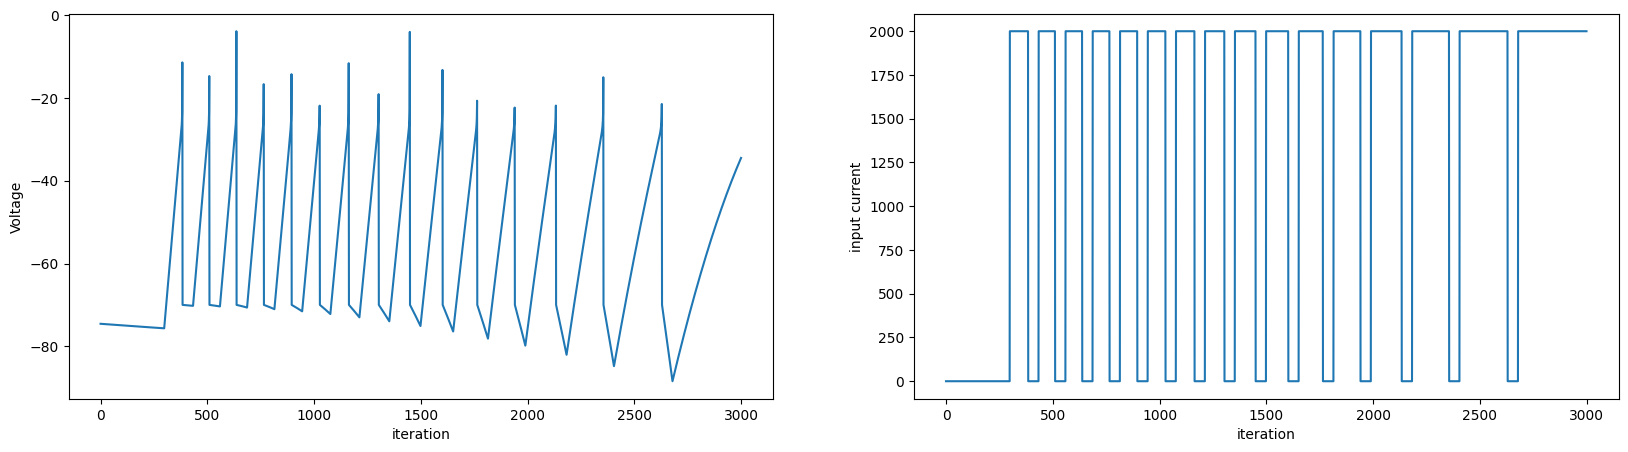
\includegraphics[width=0.9\textwidth]{Figs/aelif_o_s_r.png}
\caption{تغییرات پتانسیل مدل نورونی \lr{AELIF}
با جریان تک پله ای }
\end{figure}
\end{center}


\begin{figure}[H]
\centering
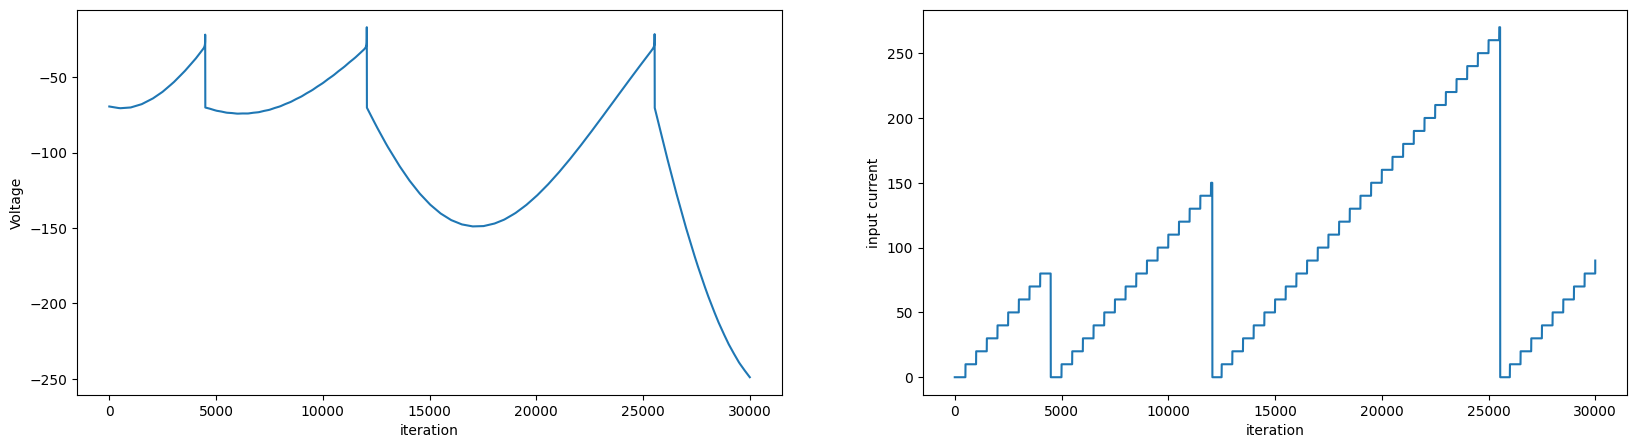
\includegraphics[width=0.9\textwidth]{Figs/aelif_s_r.png}
\caption{تغییرات پتانسیل مدل نورونی \lr{AELIF}
با جریان پله‌ای }
\end{figure}
\end{center}


\begin{figure}[H]
\centering
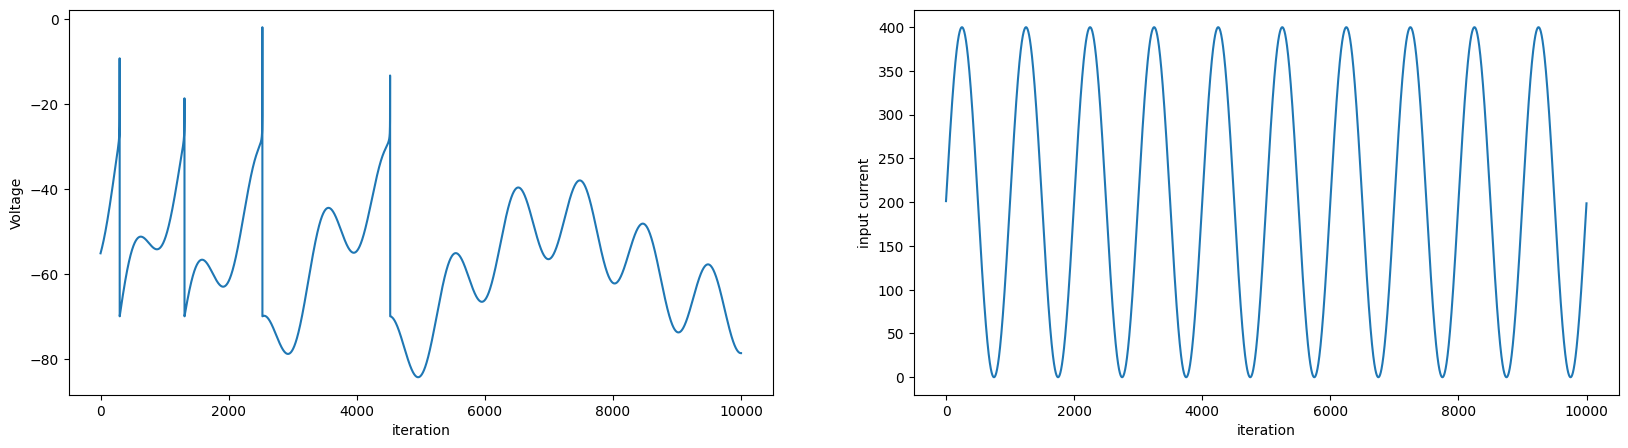
\includegraphics[width=0.9\textwidth]{Figs/aelif_sin_r.png}
\caption{تغییرات پتانسیل مدل نورونی \lr{AELIF}
با جریان سینوسی }
\end{figure}
\end{center}

\begin{figure}[H]
\centering
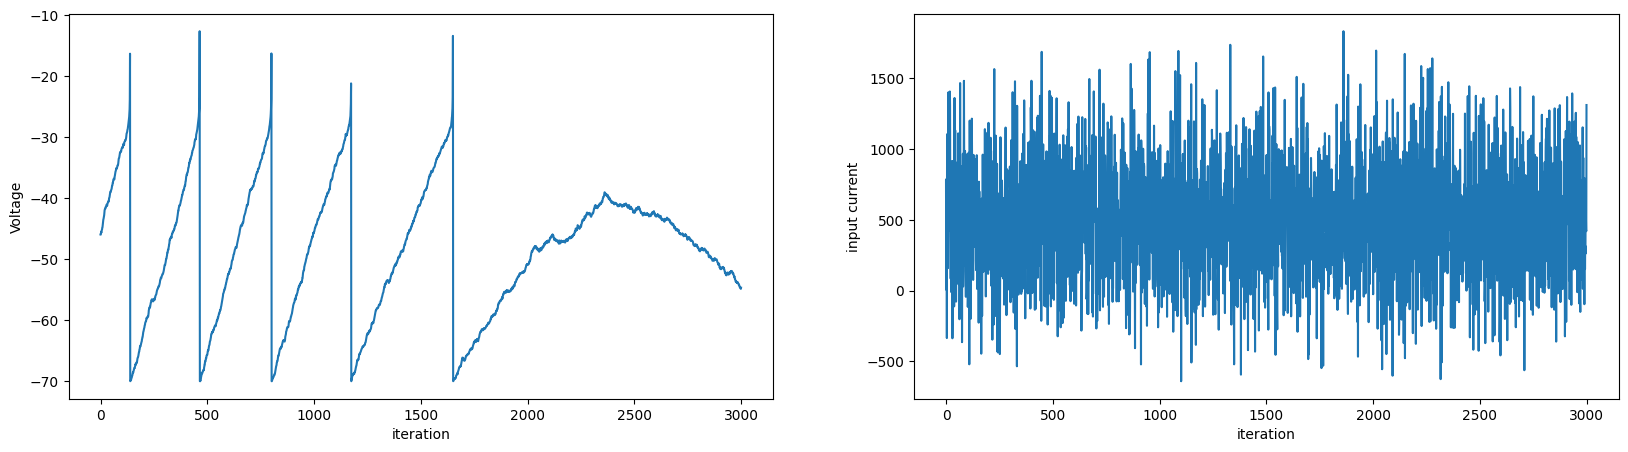
\includegraphics[width=0.9\textwidth]{Figs/aelif_n_g_r.png}
\caption{تغییرات پتانسیل مدل نورونی \lr{AELIF}
با جریان نویزی با توزیع نرمال }
\end{figure}
\end{center}


\begin{figure}[H]
\centering
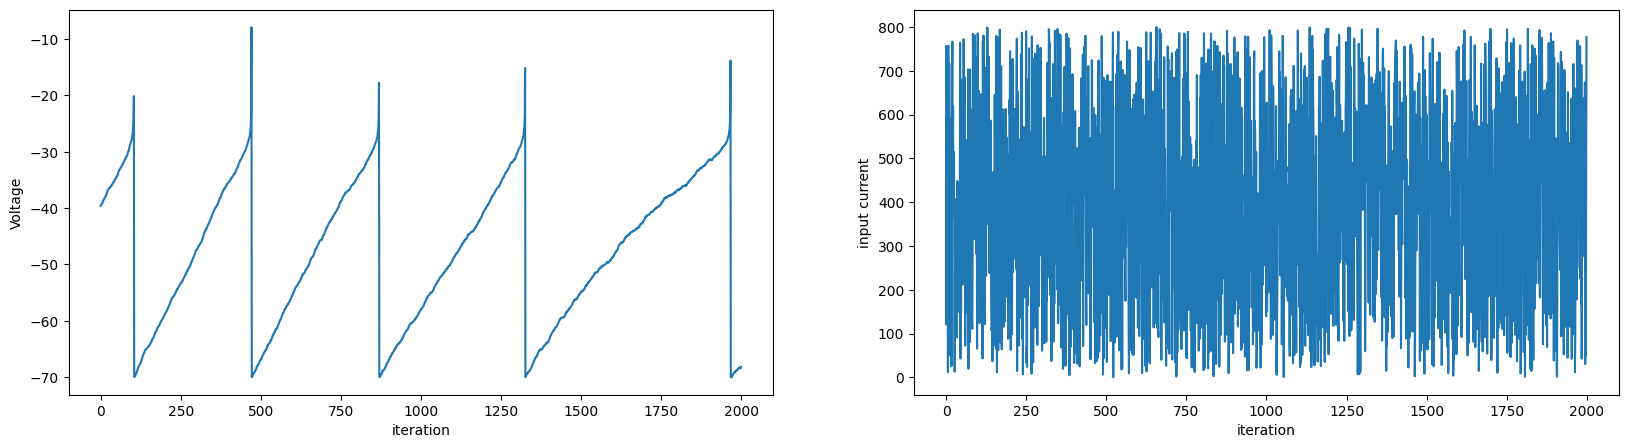
\includegraphics[width=0.9\textwidth]{Figs/aelif_n_u_r.png}
\caption{تغییرات پتانسیل مدل نورونی \lr{AELIF}
با جریان نویزی با توزیع یکنواخت }
\end{figure}
\end{center}


\section*{ه}

\subsection*{مدل نورنی \lr{LIF}}

می‌دانیم که معادله مدل نورونی \lr{LIF} عبارت است از:

$$ \tau*\frac{du}{dt} = -(u - u_{rest}) + R \times I(t) $$ 

که خب همانطور که می‌دانید پارامتر‌های متفاوتی وجود دارند که می‌توانیم برای این مدل مورد بحث قرار دهیم که هر کدام را صورت مجزا مورد تحلیل قرار می‌دهیم و در صورت نیاز نمودارهای آن‌ها را ارائه می‌دهیم:

\begin{itemize}

\item[•] \textbf{\lr{dt}}:
این پارامتر رزلوشن را نشان می‌دهد که خب هر چه قدرت محاسباتی بیشتری داشته باشیم و بخواهیم مدل دقیق تری داشته باشیم می‌توانم آن را کوچک‌تر کنیم اما به صورت معمول در این پروژه مقادیر یک‌صدم یا یک‌هزارم داشته است.

\item[•] \textbf{$\mathbf{u_{rest}}$}:
این عدد اندازه پتانسیل نورون را در حالت استراحت نشان می‌دهد که معمولا برای نورون‌های واقعی عدد منفی ۶۵ است که ما در اینجا هم از همین مقدار استفاده کرده‌ایم.

\item[•] $\mathbf{R}$:
زمانی که مدل نورنی \lr{LIF} را ارائه دادیم، گفتیم که مقاومت برای ما نقش کانال‌های یونی را بازی خواهد کرد، الان با افزایش و کاهش آن می‌تولنیم تاثیرش را بر مدل ببینیم:

برای این کار فرض می‌کنیم که جریان پله‌ای است.

\begin{figure}[H]
\centering
  \begin{subfigure}[b]{0.45\textwidth}
    \includegraphics[width=\textwidth]{Figs/lif_R=1.png}
    \caption{$R=1$}
  \end{subfigure}
  \hfill
  \begin{subfigure}[b]{0.45\textwidth}
    \includegraphics[width=\textwidth]{Figs/lif_R=10.png}
    \caption{$R=10$}
  \end{subfigure}
	\hfill
  \begin{subfigure}[b]{0.45\textwidth}
    \includegraphics[width=\textwidth]{Figs/lif_R=20.png}
    \caption{$R=20$}
  \end{subfigure}
  \caption{تغییرات اختلاف پتانسیل مدل نورونی \lr{LIF}
  با مقادیر مقاومت متفاوت
  }
\end{figure}
\end{center}

همانطور که مشاهده می‌کنید اگر جریان های یکسانی را به نورون بدهیم و هر چه مقدار $R$ را بیشتر می‌کنیم، نورون با سرعت بیشتر ضربه خواهد زد و به طور کلی با سرعت بیشتری تغییرات اختلاف پتانسیل رخ می‌دهد، به نوعی به صورتی زیستی می‌توان آن را با این عبارت که سرعت عملکرد کانال‌های یونی بیشتر و بیشتر می‌شود توجیه کرد.
 
\item[•] $\mathbf{\tau}$:
در این قسمت نیز جریان ورودی را همان جریان ثابت پله‌ای در نظر میگیریم و میزان این پارامتر را تغییر می‌دهیم و اثراتش را تحلیل می‌کنیم.


همانطور که در شکل \ref{fig:lif_tau} مشاهده می‌کنید این پارامتر عکس پارامتر $R$ عمل می‌کند به طوری که هر چه مقدار بزرگتری برای آن در نظر بگیریم نورون ضربه های کمتری می‌زند و بازه میان ضربه ها نیز بزرگتر می‌شود.

\begin{figure}[H]
\centering
  \begin{subfigure}[b]{0.45\textwidth}
    \includegraphics[width=\textwidth]{Figs/lif_tau=1.png}
    \caption{$\tau=1$}
  \end{subfigure}
  \hfill
  \begin{subfigure}[b]{0.45\textwidth}
    \includegraphics[width=\textwidth]{Figs/lif_tau=10.png}
    \caption{$\tau=10$}
  \end{subfigure}
	\hfill
  \begin{subfigure}[b]{0.45\textwidth}
    \includegraphics[width=\textwidth]{Figs/lif_tau=20.png}
    \caption{$\tau=20$}
  \end{subfigure}
  \caption{تغییرات اختلاف پتانسیل مدل نورونی \lr{LIF}
  با مقادیر $\tau$ متفاوت
  }
  \label{fig:lif_tau}
\end{figure}
\end{center}

\end{itemize}


\subsection*{مدل نورنی \lr{ELIF}}

می‌دانیم که معادله این مدل عبارت است از:

$$ \tau*\frac{du}{dt} = -(u - u_{rest}) + \Delta_{T} \exp^{\frac{u-\theta_{rh}}{\Delta_{T}}} + R \times I(t) $$

بنابراین پارامترهایی که به مدل اضافه شدند را مورد بحث و تحلیل قرار می‌دهیم:

 \begin{itemize}
 \item[•] $\mathbf{\Delta_{T}}$:
 فرض می‌کنیم که جریان ورودی مدل ما جریان پله‌ای است، سپس میزان $\Delta_{T}$ 
 را تغییر می‌دهیم و تاثیر آن را بررسی می‌کنیم.
 
 \begin{figure}[H]
\centering
  \begin{subfigure}[b]{0.45\textwidth}
    \includegraphics[width=\textwidth]{Figs/elif_delta_t=1.png}
    \caption{$\Delta_T=1$}
  \end{subfigure}
  \hfill
  \begin{subfigure}[b]{0.45\textwidth}
    \includegraphics[width=\textwidth]{Figs/elif_delta_t=10.png}
    \caption{$\Delta_T=10$}
  \end{subfigure}
  \caption{تغییرات اختلاف پتانسیل مدل نورونی \lr{ELIF}
  با مقادیر $\Delta_{T}$ متفاوت
  }
  \label{fig:elif_delta_t}
\end{figure}
\end{center}
 
 همانطور که در شکل \ref{fig:elif_delta_t} مشاهده می‌کنید مقدار $\Delta_T$ رابطه عکس با سرعت نمایی رشد اختلاف پتانسیل در لحظات پتانسیل فعالیت را دارد، هرچقدر که مقدار کوچکتری داشته باشد با سرعت نمایی بیشتری این تغییر رخ می‌دهد و اگر که آن را بزرگتر کنیم این نرخ کمتر می‌شود.
 
 \item[•] $\theta_{rh}$: 
 همانطور که راجب این پارامتر قبلا هم صحبت کردیم، این پارامتر در واقع تعیین کننده حد آستانه ما است، بعد از رسیدن به این مقدار اختلاف پتانسیل نورون به صورت نمایی کم می‌شود و بعد از این موقع پتانسیل فعالیت شبیه سازی می‌شود، بنابراین به نوعی ما دو حد آستانه داریم که از حد آستانه دیگر برای تنظیم مجدد پتانسیل استفاده می‌کنیم.
 \end{itemize}

\subsection*{مدل نورنی \lr{AELIF}}

می‌دانیم که معادله این مدل نورونی عبارت است از:

$$ \tau_m*\frac{du}{dt} = -(u - u_{rest}) + \Delta_{T} \exp^{\frac{u-\theta_{rh}}{\Delta_{T}}} - R \sum_k w_k + R \times I(t) $$

$$ \tau_k*\frac{dw_k}{dt} = a_k (u - u_{rest}) - w_k + b_k \tau_k \sum_{t^f} \delta(t-t^f)$$

همانطور که معادلات را مشاهده می‌کنید پارامترهای مدل نورنی تغییر نداشته اما برای اینکه خاصیت تطبیق پذیری را به مدل اضافه کنیم، یک وزنی را همواره از اختلاف پتانسیل کم می‌کنیم که پارامتر های آن را مورد بحث قرار می‌دهیم.

\begin{itemize}
\item[•] $\mathbf{\tau_k}$:
یک جریان ثابت را به نورون ورودی می‌دهیم و مقدار $\tau_k$ را تغییر می‌دهیم تا تاثیر آن را مورد تحلیل قرار دهیم:

\begin{figure}[H]
\centering
  \begin{subfigure}[b]{0.45\textwidth}
    \includegraphics[width=\textwidth]{Figs/aelif_tau_k=1}
    \caption{$\tau_k=1$}
  \end{subfigure}
  \hfill
  \begin{subfigure}[b]{0.45\textwidth}
    \includegraphics[width=\textwidth]{Figs/aelif_tau_k=10}
    \caption{$\tau_k=10$}
  \end{subfigure}
	\hfill
  \begin{subfigure}[b]{0.45\textwidth}
    \includegraphics[width=\textwidth]{Figs/aelif_tau_k=100}
    \caption{$\tau_k=100$}
  \end{subfigure}
  \caption{تغییرات اختلاف پتانسیل مدل نورونی \lr{AELIF}
  با مقادیر $\tau_k$ متفاوت
  }
\end{figure}
\end{center}


\begin{figure}[H]
\centering
  \begin{subfigure}[b]{0.3\textwidth}
    \includegraphics[width=\textwidth]{Figs/aelif_tau_k=1_s.png}
    \caption{$\tau_k=1$}
  \end{subfigure}
  \hfill
  \begin{subfigure}[b]{0.3\textwidth}
    \includegraphics[width=\textwidth]{Figs/aelif_tau_k=10_s.png}
    \caption{$\tau_k=10$}
  \end{subfigure}
	\hfill
  \begin{subfigure}[b]{0.3\textwidth}
    \includegraphics[width=\textwidth]{Figs/aelif_tau_k=100_s.png}
    \caption{$\tau_k=100$}
  \end{subfigure}
  \caption{ زمان ضربه 
    با مقادیر $\tau_k$ متفاوت}
\end{figure}
\end{center}


همانطور که مشاهده می‌کنید هر چه اندازه $\tau_k$ را افزایش می‌دهیم میزان تطبیق پذیری نورون افزایش می‌یابد و همچنین نرخ ضربه به طور کلی کاهش می‌یابد.

\item[•] $\mathbf{a_k}$:
می‌دانیم که ترم $a_k(u - u_{rest})$ نشان می‌دهد که میزان اختلاف ما از از حالت استراحت در میزان تطبیق پذیری می‌تواند مهم باشد که خب با استفاده از $a_k$ می‌توانیم این تاثیر را کم یا زیاد کنیم.


یک جریان ثابت را به نورون ورودی می‌دهیم و مقدار $a_k$ را تغییر می‌دهیم تا تاثیر آن را مورد تحلیل قرار دهیم:

\begin{figure}[H]
\centering
  \begin{subfigure}[b]{0.3\textwidth}
    \includegraphics[width=\textwidth]{Figs/aelif_a_k=1.png}
    \caption{$a_k=1$}
  \end{subfigure}
  \hfill
  \begin{subfigure}[b]{0.3\textwidth}
    \includegraphics[width=\textwidth]{Figs/aelif_a_k=10.png}
    \caption{$a_k=10$}
  \end{subfigure}
	\hfill
  \begin{subfigure}[b]{0.3\textwidth}
    \includegraphics[width=\textwidth]{Figs/aelif_a_k=100.png}
    \caption{$a_k=100$}
  \end{subfigure}
  \caption{ زمان ضربه 
    با مقادیر $a_k$ متفاوت}
\label{fig:aelif_a_k}
\end{figure}
\end{center}


همانطور که در شکل \ref{fig:aelif_a_k} مشاهده می‌کنید، هر چه مقدار $a_k$ را بیشتر می‌کنیم نتنها خاصیت تطبیق پذیری خیلی می‌تواند زیادتر شود بلکه باعث می‌شود که نورن خیلی از حالت استراحت خود دور نشود و همواره در اطراف آن بازی کند و به حد آستانه نرسد.


 این پارمتر با پارامتر بعدی رابطه مهمی دارد، به طوری که اگر $b_k$ خیلی عدد بزرگتری نسبت به این پارامتر باشد آنگاه در مدت زمان طولانی خاصیت تطبیق پذیری به سرعت افزایش می‌یابد اما این ترم آنقدر قوی نیست که جلوی کم شدن اندازه اختلاف پتانسیل را بگیرد تا جایی که حتی پتانسیل نورون به منفی بی نهایت میل خواهد کرد. بنابراین می‌توان گفت که این وزن تاثیر مهمی در حفظ تعادل نورون در زمانی که به یک ورودی عادت می‌کند دارد.


\item[•] $\mathbf{b_k}$:
می‌دانیم که زمانی که ضربه داریم مقدار $b_k$ به وزن اضافه می‌شود بنابراین این پارامتر مهمی در تعیین میزان تطبیق پذیری نورن می‌باشد.
 
یک جریان ثابت را به نورون ورودی می‌دهیم و مقدار $b_k$ را تغییر می‌دهیم تا تاثیر آن را مورد تحلیل قرار دهیم:

\begin{figure}[H]
\centering
  \begin{subfigure}[b]{0.45\textwidth}
    \includegraphics[width=\textwidth]{Figs/aelif_b_k=1}
    \caption{$b_k=1$}
  \end{subfigure}
  \hfill
  \begin{subfigure}[b]{0.45\textwidth}
    \includegraphics[width=\textwidth]{Figs/aelif_b_k=20}
    \caption{$b_k=20$}
  \end{subfigure}
	\hfill
  \begin{subfigure}[b]{0.45\textwidth}
    \includegraphics[width=\textwidth]{Figs/aelif_b_k=40}
    \caption{$b_k=40$}
  \end{subfigure}
  \caption{تغییرات اختلاف پتانسیل مدل نورونی \lr{AELIF}
  با مقادیر $b_k$ متفاوت
  }
\end{figure}
\end{center}

همانطور که بالاتر اشاره کردیم، این پارامتر نقش مهمی در تعیین میزان تطبیق پذیری نورون دارد و اگر مقدار آن را افزایش دهیم میزان تطبیق پذیری نورون افزایش می‌یابد و از جایی به بعد اجازه ضربه را به نورون نمی‌دهد اما نمی‌توان راجب این پارامتر هم به تنهایی نظر داد چون مقدار $a_k$ تاثیر مهمی در رفتار این پارامتر دارد همانطور که در بخش قبل توضیح دادیم.



\section*{نتیجه گیری}

در این پروژه سه مدل نورنی متفاوت را پیاده سازی و تحلیل کردیم و شناخت بهتری نسبت به نقش هر یک از پارامترهای مدل‌ها پیدا کردیم، در ادامه نیز قصد داریم که با آن‌ها یک شبکه عصبی تشیل دهیم که به این نتایج بدست آمده نیاز خواهیم داشت.




\end{itemize}
\end{document}
